\chapter{Results}\label{ch:results}
In this chapter, a simulation of the northern part of Fredericia will be conducted.}

The goal of this simulation is to simulate a daily flow in the northern part of Fredericia.%, where the disturbance can be seen on the input to the WWTP. 
For this purpose the simulation environment explained in chapter \ref{ch:simulation} is utilized. The pumping station, illustrated with the blue dot in figure \ref{fig:kloakgrid_simplified}, is not included in this simulation, the reason is that it will have a dampening effect on the disturbances from the larger industry and the surrounding urban areas. 
%as it will smooth the flow from that point and into the WWTP, thus there will not be any variation in the flow into the WWTP. 
To generate the disturbances from the residential and industrial areas, shown in figure \ref{fig:kloakgrid_simplified}, the flow profiles in appendix \ref{app:flow_profiles} is used. These disturbance models are not simulated in pipes from the various areas into the main sewer line but are directly added into the main sewer line. Therefore the results are expected to have higher peaks, as these models are not attenuated, as they would have been if they were simulated in pipes from the various areas. It has been chosen to only use the disturbance from the brewery and bottling plant, as the data from the refinery weren't available. The disturbances from the brewery and bottling plant is shown in figure \ref{fig:flow_profile_industry}. The pipe specifications for this simulation can be seen in table \ref{tab:pipe_data_nonlinear_linear_testv2}.  
\begin{table}[H]
\centering
\begin{tabular}{|c|c|c|c|c|c|c|c|c|}
\hline
	\rowcolor[HTML]{9B9B9B} 
\begin{tabular}[c]{@{}c@{}}Component\\ number\end{tabular} & Length {[}m{]} & Sections & Dx {[}m{]} & $S_b$     & d {[}m{]} & $\theta$ & \begin{tabular}[c]{@{}c@{}}$Q_f $\\  {[}$m^3/s${]}\end{tabular} & \begin{tabular}[c]{@{}c@{}}$side$\\  inflow\end{tabular} \\ \hline
1                                                          & 700            & 35       & 20         & 0,003  & 0,9       & 0,65     & 0,973    	&0            \\ \hline
3                                                          & 303            & 15       & 20,2       & 0,003  & 0,9       & 0,65     & 0,973     &0            \\ \hline
4                                                          & 27             & 2        & 13,5       & 0,003  & 1         & 0,65     & 1,284     &1          \\ \hline
5                                                          & 155            & 8        & 19,4       & 0,0041 & 1         & 0,65     & 1,50      &0            \\ \hline
6                                                          & 295            & 14       & 21         & 0,0122 & 0,8       & 0,65     & 1,438     &0           \\ \hline
7                                                          & 318            & 15       & 21,2       & 0,0053 & 0,9       & 0,65     & 1,293     & 1        \\ \hline
8                                                          & 110            & 5        & 22         & 0,0036 & 0,9       & 0,65     & 1,066     &1        \\ \hline
9                                                          & 38             & 2        & 19         & 0,0024 & 1         & 0,65     & 1,149     &1         \\ \hline
10                                                         & 665            & 30       & 22,2       & 0,003  & 1         & 0,65     & 1,284     &1        \\ \hline
11                                                         & 155            & 7        & 22,1       & 0,0008 & 1         & 0,65     & 0,663     &0         \\ \hline
12                                                         & 955            & 47       & 20,3       & 0,0029 & 1,2       & 0,65     & 2,041     &1         \\ \hline
13                                                         & 304            & 15       & 20,3       & 0,003  & 1,2       & 0,65     & 2,076     &0         \\ \hline
14                                                         & 116            & 5        & 23,2       & 0,0021 & 1,2       & 0,65     & 1,737     &1         \\ \hline
15                                                         & 283            & 12       & 23,6       & 0,0017 & 1,4       & 0,65     & 2,346     &1          \\ \hline
16                                                         & 31             & 2        & 15,5       & 0,0019 & 1,4       & 0,65     & 2,480     &1          \\ \hline
17                                                         & 125            & 6        & 20,8       & 0,0021 & 1,6       & 0,65     & 3,707     &0          \\ \hline
18                                                         & 94             & 4        & 23,5       & 0,0013 & 1,5       & 0,65     & 2,461     &0             \\ \hline
19                                                         & 360            & 18       & 20         & 0,0046 & 1,6       & 0,65     & 5,487     &1           \\ \hline
21                                                         & 736            & 38       & 19,4         & 0,0012 & 1,6       & 0,65     & 2,802   &0          \\ \hline
\end{tabular}
\caption{Specification of pipes used in the final simulation.}
\label{tab:pipe_data_nonlinear_linear_testv2}
\end{table}

The tank specifications can be seen in table \ref{tab:tank_data_nonlinear_linear_testv2}.

\begin{table}[H]
\centering
\begin{tabular}{|c|c|c|}
\hline
\begin{tabular}[c]{@{}c@{}}Part\end{tabular} & 2 (Tank)  & 20 (Tank)\\ \hline
Size $[m^3]$                                              & 90 & 90\\ \hline
Height {[}m{]}                                             & 10 & 10\\ \hline
Area $[m^2]$                                              & 9  & 9\\ \hline
$Q_{out_{max}}$ $[m^3/s]$                                      & 0.973  & 2.80\\ \hline
\end{tabular}
\caption{Tank specification for the final simulation. }
\label{tab:tank_data_nonlinear_linear_testv2}
\end{table}

Furthermore, table \ref{tab:system_setup_nonlinear_linear_testv2} show the system setup.

\begin{table}[H]
\centering
\begin{tabular}{|c|c|c|}
\hline
	\rowcolor[HTML]{9B9B9B} 
Type  & Component & Sections \\ \hline
Pipe  & 1         & 35       \\ \hline
Tank  & 1         & 1        \\ \hline
Pipe  & 17        & 207      \\ \hline
Tank  & 1         & 1        \\ \hline
Pipe  & 1         & 38        \\ \hline
Total & 21        & 282      \\ \hline
\end{tabular}
\caption{The system setup.}
\label{tab:system_setup_nonlinear_linear_testv2}
\end{table}

The first component in the setup of the sewer network is a pipe followed by a tank where after 18 pipes follows. The first pipe and the two tanks have been added to the original sewer network shown in figure \ref{fig:sewer_line_diagram}. The first pipe is connected from the larger industrial area to the main sewer line indicated by a black circle in figure \ref{fig:kloakgrid_simplified}, where the first tank is placed as well. The reason for placing the tank there is, that it should be able to smoothen the flow of wastewater coming from the larger industry. Furthermore, the pipe is placed, such that the MPC should be able to use the delay for prediction.%, as it would be able to measure the disturbance going into the pipe at the industry, and thereby use it in the predictive model to calculate the most optimal control output to the pump. 
 However, as this is not possible, due to the problems experienced with the MPC controller,% not able to keep a flow output, where the flow variations are kept to a minimum, and as the prediction horizon is limited due to non-convexity 
as explained in section \ref{se:model_predictive_control}. 

The second tank is placed just before the WWTP with the purpose of smoothening the flow into the WWTP. %However, in this simulation, the tanks will just transfer wastewater from the previous pipe to the pipe after the tank, due to the MPC controller is not able to control them optimally. 
Due to the lack of a controller the tanks is given a static input during the simulation.
%Furthermore several simulations were conducted to obtain an optimal $\Delta t$ as explained in section \ref{subse:stability_and_precision}. As the pipes are split into different sections and as the average flow height is also different from pipe to pipe, the Courant number varies from pipe to pipe. Thus it is difficult to tune so all pipes have the most optimal Courant number. However, it was found that a $\Delta t = 20$, with the given $\Delta x$ shown in table \ref{tab:pipe_data_nonlinear_linear_testv2} for the various pipes, gave an output, where distortion was visible.


In figure \ref{fig:simulation_output_first} the output of a simulated period of two days can be seen. 

\begin{figure}[H]
\centering
% This file was created by matlab2tikz.
%
%The latest updates can be retrieved from
%  http://www.mathworks.com/matlabcentral/fileexchange/22022-matlab2tikz-matlab2tikz
%where you can also make suggestions and rate matlab2tikz.
%
\definecolor{mycolor1}{rgb}{0.00000,0.44700,0.74100}%
%
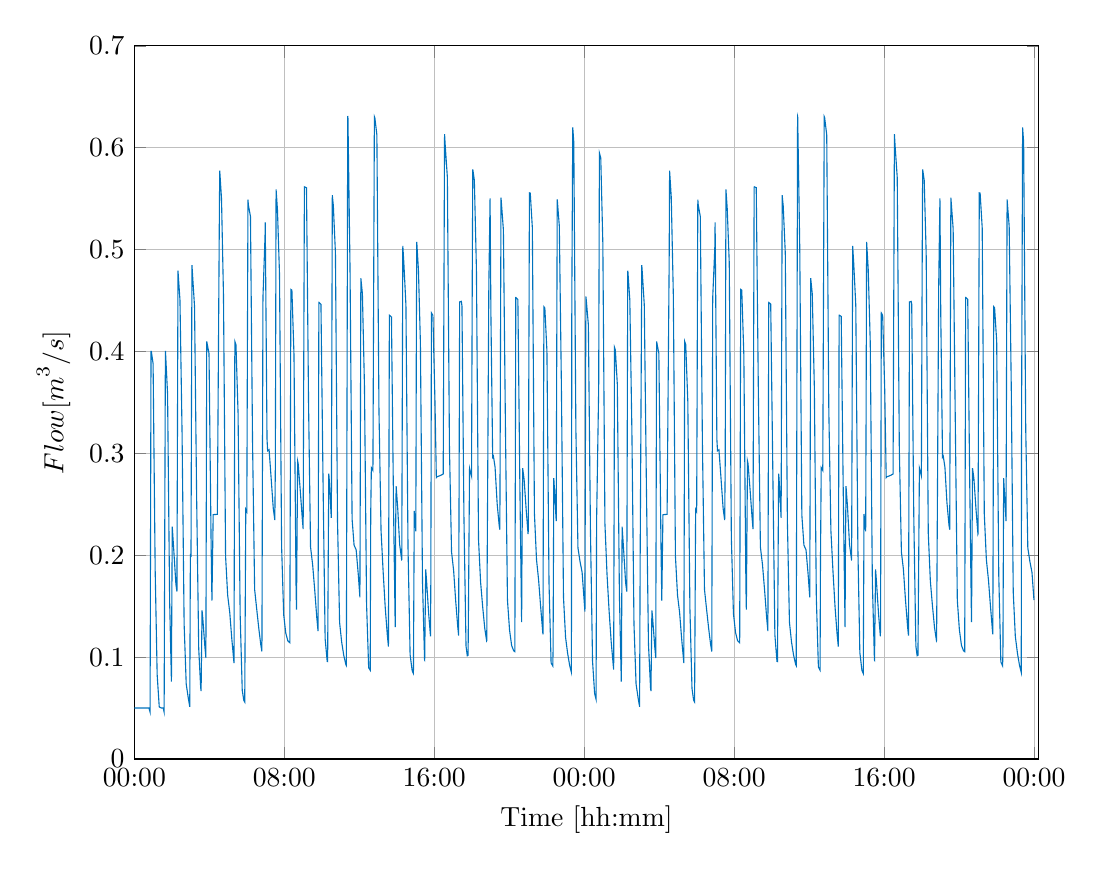
\begin{tikzpicture}

\begin{axis}[%
width=4.521in,
height=3.566in,
at={(0.758in,0.481in)},
scale only axis,
xmin=1,
scaled x ticks = false,
xmajorgrids,
ymajorgrids,
xmax=173664,
xtick={1,28801,57601,86401,115201,144001,172801},
xticklabels={{00:00},{08:00},{16:00},{00:00},{08:00},{16:00},{00:00},{},{},{}},
xlabel={Time [hh:mm]},
ymin=0,
ymax=0.7,
ylabel={$\text{Flow [m}^\text{3}\text{/s]}$},
axis background/.style={fill=white}
]
\addplot [color=mycolor1,solid,forget plot]
  table[row sep=crcr]{%
1	0.0499997152763342\\
381	0.0499999892074085\\
681	0.0499999887402718\\
781	0.0499999900942177\\
801	0.0499999900283255\\
1081	0.049999984018313\\
1261	0.0499999893262727\\
1521	0.0499999838340426\\
1601	0.049999984809447\\
2001	0.0499999906588171\\
2061	0.0499999922125646\\
2401	0.049999988996632\\
2781	0.0499999918475296\\
2801	0.0499999801986038\\
3021	0.0460373492555953\\
3201	0.39999620912548\\
3261	0.399999964024236\\
3601	0.388038894071086\\
4001	0.184947858626601\\
4381	0.082805088531536\\
4781	0.0511451879298567\\
5181	0.0500002487860619\\
5541	0.0499999248577416\\
5721	0.0460373452553259\\
5961	0.399999974821009\\
5981	0.399999971271513\\
6381	0.358516455127467\\
6781	0.154383868746348\\
7121	0.0760256189325568\\
7181	0.13826974014641\\
7281	0.228026620985396\\
7581	0.204239805785136\\
7981	0.171590440555943\\
8181	0.164315181527722\\
8381	0.47926934050765\\
8761	0.450413278243777\\
9161	0.321534576651487\\
9561	0.132277730995904\\
9961	0.0735649221955217\\
10361	0.0597071439387407\\
10641	0.0512695775424259\\
10761	0.20005447478489\\
10881	0.199434615905679\\
11061	0.48473586623314\\
11161	0.476723871738909\\
11561	0.443897750738214\\
11961	0.25806849480281\\
12361	0.108844325174995\\
12741	0.0700275093087758\\
12821	0.0667206908995504\\
13001	0.145928679109392\\
13141	0.138393729441425\\
13541	0.110667079625233\\
13741	0.0991507389943454\\
13901	0.40986305875768\\
13941	0.40882623802115\\
14341	0.398007217901318\\
14741	0.212131825065823\\
14901	0.155368306478837\\
15141	0.239872608579426\\
15541	0.240004691937102\\
15941	0.240038886655287\\
16341	0.543707035296884\\
16401	0.577386156049016\\
16741	0.5499489464615\\
17121	0.454515865313659\\
17521	0.199211784759613\\
17921	0.160813386913845\\
18321	0.143916888943139\\
18721	0.117703671201611\\
19121	0.095049498732015\\
19141	0.0940665657039142\\
19301	0.409784435964215\\
19521	0.406501876116627\\
19921	0.33935537668123\\
20321	0.141804797058712\\
20721	0.067435176520201\\
21021	0.0575846925747079\\
21201	0.0559457131457851\\
21401	0.244991184003057\\
21601	0.242763538199487\\
21821	0.5490148580277\\
21901	0.543815970276843\\
22301	0.532449053725931\\
22701	0.311242442063504\\
23101	0.166455067970211\\
23501	0.147143722635203\\
23901	0.128218569971245\\
24301	0.111515660096113\\
24501	0.105546274424128\\
24701	0.452877166239096\\
25101	0.513490813859022\\
25141	0.526641040406919\\
25481	0.314069608587414\\
25601	0.302486128983783\\
25881	0.303568709699798\\
26281	0.275044058907798\\
26681	0.245964195626756\\
26981	0.234447696691942\\
27081	0.288110624118585\\
27221	0.559006245862765\\
27481	0.539613674285018\\
27881	0.475567692570443\\
28281	0.209018911404775\\
28681	0.141668747218986\\
29081	0.123608641874535\\
29481	0.11592694443507\\
29861	0.114080220104003\\
30061	0.460896204122244\\
30261	0.460167448207798\\
30661	0.396678419054452\\
31061	0.168157104268696\\
31141	0.146550603859365\\
31361	0.292440612392119\\
31461	0.290155884720642\\
31861	0.26381450895376\\
32261	0.23554830781087\\
32421	0.225714221407563\\
32661	0.561584147546688\\
33061	0.560624758930501\\
33461	0.348105695677251\\
33841	0.208065283311125\\
34241	0.190782917669544\\
34641	0.166025134280847\\
35041	0.13873822553377\\
35281	0.125451644802619\\
35441	0.4478352243038\\
35461	0.44811407769246\\
35841	0.446214141629251\\
36241	0.27225617680166\\
36641	0.118110855826106\\
37041	0.095767561962741\\
37121	0.0956553614348974\\
37341	0.280096449864026\\
37441	0.273855912758517\\
37821	0.236596990821348\\
37841	0.237774941596493\\
38021	0.553366894967955\\
38221	0.54291518952707\\
38621	0.49660305179753\\
39021	0.233847581211315\\
39421	0.134033881707084\\
39821	0.114649017608518\\
40221	0.101701052031103\\
40621	0.0927146992547936\\
40721	0.0917383187540116\\
40981	0.63107071951054\\
41021	0.630035704702444\\
41421	0.482341851596278\\
41821	0.235563366290832\\
42201	0.209832049584584\\
42601	0.205284923234108\\
43001	0.181573721441432\\
43321	0.158651139798747\\
43401	0.287395033266756\\
43501	0.471956377710797\\
43801	0.456578916341174\\
44201	0.364798527107059\\
44601	0.151919551074707\\
45001	0.0895967214260026\\
45301	0.0871144475971674\\
45401	0.241707281322062\\
45521	0.285948268035892\\
45821	0.283146889932263\\
46101	0.630469173265171\\
46201	0.629088537957435\\
46581	0.612545920500935\\
46981	0.342528955023114\\
47381	0.224203484709649\\
47781	0.184153073081266\\
48181	0.149030782566006\\
48581	0.12195593910867\\
48801	0.110280587955104\\
48981	0.435567061037672\\
49381	0.433837256348174\\
49781	0.247137117278272\\
50101	0.129323544894529\\
50181	0.226587016813804\\
50281	0.267899772040847\\
50581	0.246318904302867\\
50961	0.210314398331763\\
51341	0.195657253277077\\
51361	0.195784009404707\\
51561	0.503592036774015\\
51761	0.486974841272141\\
52161	0.445428690023276\\
52561	0.207716541625214\\
52961	0.102502304765683\\
53361	0.0865204262570826\\
53601	0.0839471479111217\\
53761	0.243524692542883\\
54061	0.22335472358936\\
54161	0.413641605154435\\
54241	0.507566556159231\\
54561	0.48007415997152\\
54941	0.408444008474248\\
55341	0.174114153859742\\
55741	0.0971405673619263\\
55761	0.096975498915427\\
55961	0.186119510987269\\
56141	0.173353292951344\\
56541	0.141804669337536\\
56881	0.120312676919824\\
56941	0.17363089926247\\
57061	0.437782042398014\\
57341	0.435474087380637\\
57741	0.350377749978731\\
58001	0.276216298585415\\
58141	0.277039370834222\\
58541	0.277740752111343\\
58941	0.278635286488113\\
59321	0.279736664395953\\
59581	0.613239888945005\\
59721	0.601155920090224\\
60121	0.570829618399022\\
60521	0.30525522703366\\
60921	0.203256919582693\\
61321	0.185129585157137\\
61721	0.154979527639579\\
62121	0.129229876043253\\
62281	0.12114747426953\\
62481	0.44862995078268\\
62801	0.449171273418054\\
62921	0.444677955276041\\
63301	0.237964284751834\\
63701	0.111008795041031\\
63941	0.101319095647373\\
64101	0.101831871303562\\
64381	0.285451159479523\\
64761	0.277800728120848\\
64901	0.472346688429331\\
65001	0.578732309508892\\
65301	0.568128800263333\\
65701	0.480556114992309\\
66101	0.215435701651473\\
66501	0.173587977353262\\
66901	0.149411121057409\\
67301	0.128194088457934\\
67661	0.115879979337036\\
67681	0.116080976474654\\
68081	0.463231310412606\\
68321	0.550240918542084\\
68481	0.43704169328213\\
68821	0.296195131686067\\
68961	0.297296204143991\\
69281	0.286349521684829\\
69681	0.250540179409776\\
70081	0.228693231365457\\
70201	0.225059553792036\\
70421	0.550888655859785\\
70481	0.546993291279657\\
70881	0.519239767321056\\
71281	0.321893080651539\\
71661	0.155884099827311\\
72061	0.126611870338134\\
72461	0.111441871585865\\
72861	0.106140611089357\\
73081	0.105332967336101\\
73261	0.452946083990718\\
73281	0.453024300871342\\
73661	0.451074937198832\\
74061	0.26082900810748\\
74381	0.134237338321971\\
74461	0.207813944879953\\
74581	0.285378186391529\\
74861	0.274285223507388\\
75261	0.244391347849864\\
75621	0.220651866001535\\
75661	0.224809763811749\\
75881	0.5556579938168\\
76041	0.555440125466322\\
76441	0.52143634234302\\
76841	0.240745754972094\\
77241	0.195680996475161\\
77641	0.175811605109868\\
78041	0.149008733822511\\
78441	0.124162090755598\\
78481	0.122293389503727\\
78661	0.44384907080836\\
78841	0.442708151044371\\
79241	0.400372910545192\\
79641	0.172855897377427\\
80041	0.0943411879687305\\
80361	0.0913677029693039\\
80421	0.105748914607317\\
80561	0.275622277873239\\
81021	0.233525034544167\\
81221	0.549299988830962\\
81621	0.523015869588244\\
82021	0.365589134600443\\
82421	0.158832345842062\\
82821	0.119381319389791\\
83221	0.103510284822917\\
83621	0.0914259162743653\\
83941	0.0850821629137212\\
84021	0.449966203224246\\
84201	0.619938777189986\\
84401	0.605215327407337\\
84801	0.323950052106171\\
85201	0.207162769487388\\
85601	0.193722933184863\\
86001	0.183208432749678\\
86401	0.154546451194393\\
86541	0.144709226768709\\
86721	0.454054707630259\\
86801	0.450268450488853\\
87201	0.426082168190829\\
87601	0.224018825746384\\
88001	0.0961050037604321\\
88401	0.0642514476254031\\
88681	0.058588377418986\\
88781	0.233884823055304\\
89181	0.363764232190534\\
89321	0.594800267880994\\
89581	0.589951272879468\\
89981	0.505665048374919\\
90381	0.231007553197322\\
90781	0.181446768847678\\
91181	0.145374472013491\\
91581	0.115191653805948\\
91981	0.0918291899207325\\
92061	0.0877953189909785\\
92221	0.403907758239193\\
92381	0.401514711023063\\
92761	0.367814281450466\\
93161	0.161459811427181\\
93521	0.0760258697047347\\
93561	0.0969253175283628\\
93681	0.228026635800281\\
93961	0.206157068010913\\
94361	0.172716138741509\\
94581	0.164315181527722\\
94761	0.477771577804068\\
94781	0.47926934050765\\
95161	0.450413278243778\\
95561	0.321534576651487\\
95961	0.132277730995905\\
96361	0.0735649221955217\\
96761	0.0597071439387407\\
97041	0.0512695775424261\\
97141	0.189954342640788\\
97461	0.48473586623314\\
97541	0.478621526310808\\
97941	0.445565551010111\\
98341	0.270052824073967\\
98741	0.112972942133323\\
99141	0.0700275093087758\\
99221	0.0667206908995504\\
99401	0.145928679109392\\
99541	0.138393729441425\\
99941	0.110667079625233\\
100141	0.0991507389943454\\
100301	0.40986305875768\\
100341	0.40882623802115\\
100741	0.398007217901318\\
101141	0.212131825065823\\
101301	0.155368306478837\\
101521	0.239674727124832\\
101921	0.240004160488744\\
102321	0.240032761489357\\
102721	0.490613201150536\\
102801	0.577385614042946\\
103121	0.551397788492204\\
103521	0.454515521091378\\
103921	0.199211766547411\\
104321	0.160811738559319\\
104721	0.143916519077449\\
105121	0.117702397972358\\
105501	0.0960563302766093\\
105541	0.0940655608631718\\
105701	0.409782142347942\\
105901	0.406701240316587\\
106301	0.350756062230757\\
106701	0.148179236245713\\
107101	0.0692618286459731\\
107421	0.0575801460066641\\
107601	0.0559429268585551\\
107801	0.244982676605651\\
108001	0.242757068811194\\
108221	0.54900476716055\\
108301	0.543808297503321\\
108701	0.532436480925017\\
109101	0.311241030199004\\
109501	0.166447159541348\\
109881	0.14801645052783\\
110281	0.129144882903335\\
110681	0.112225593742404\\
110901	0.105541387787785\\
111081	0.452627367523953\\
111481	0.501364815585408\\
111541	0.526586805232183\\
111881	0.314064927206939\\
112001	0.302477482482032\\
112281	0.303564415396613\\
112681	0.275045931553673\\
113081	0.245964222909356\\
113381	0.234448498754518\\
113481	0.288116696094247\\
113621	0.559006398210286\\
113861	0.540979121709231\\
114261	0.486855270635058\\
114661	0.217493518570819\\
115061	0.142802563645621\\
115461	0.124291854749527\\
115861	0.116093137321325\\
116261	0.114084290390741\\
116461	0.460899377915235\\
116661	0.460171947548487\\
117061	0.396679285152434\\
117461	0.168158461755987\\
117541	0.146555138425319\\
117761	0.292445572598367\\
117861	0.290159181668251\\
118241	0.265401886805784\\
118641	0.236956301886082\\
118821	0.225714522330167\\
119041	0.561469488609575\\
119061	0.561586041554716\\
119441	0.560805439144691\\
119841	0.363932228586388\\
120241	0.208067125535311\\
120641	0.190785255682231\\
121041	0.166025588105298\\
121441	0.13873932167539\\
121681	0.125453388188775\\
121841	0.447837563995478\\
121861	0.448116051383338\\
122221	0.4464561479952\\
122621	0.284824476239217\\
123021	0.121970167931679\\
123421	0.0958081500032729\\
123521	0.0956573749864267\\
123741	0.280096851577685\\
123821	0.275531608454023\\
124221	0.236598409026601\\
124421	0.553367619300467\\
124621	0.5429157709688\\
125021	0.496603413412628\\
125421	0.233847680410384\\
125821	0.134033685469667\\
126221	0.114650333534502\\
126601	0.102289103709303\\
127001	0.0929882528747439\\
127121	0.0917392868371645\\
127381	0.631071912873843\\
127401	0.630719116657667\\
127801	0.501347161814062\\
128201	0.239397450469059\\
128601	0.209832888971714\\
129001	0.205285541414406\\
129401	0.181574246023112\\
129721	0.158651581187078\\
129801	0.287397627582394\\
129901	0.471956617871342\\
130201	0.456579492165227\\
130601	0.364798643465493\\
130981	0.158461721428025\\
131381	0.0902446213392131\\
131701	0.0871147730920042\\
131781	0.195332180975037\\
131921	0.285946978271874\\
132221	0.283146011645084\\
132501	0.630469563534361\\
132581	0.62947257325151\\
132981	0.612546279103266\\
133381	0.342529069488647\\
133781	0.22420331583186\\
134181	0.18415338411579\\
134581	0.149030236035514\\
134961	0.123132349572876\\
135201	0.110280603793395\\
135361	0.435176913377614\\
135381	0.435567198316332\\
135761	0.434402963450522\\
136161	0.258663077151003\\
136501	0.129324848709165\\
136561	0.193972315730123\\
136681	0.267900152487372\\
136961	0.248282666486158\\
137361	0.210314788420516\\
137741	0.195657673398787\\
137761	0.195784442440667\\
137961	0.503592296507298\\
138161	0.48697576182077\\
138561	0.445428205217198\\
138961	0.207716601935443\\
139341	0.104535524709347\\
139741	0.0868948301247878\\
140001	0.0839475146696737\\
140141	0.240432040289202\\
140461	0.223354613707161\\
140541	0.341067258228241\\
140641	0.507566355305644\\
140941	0.481669135095204\\
141341	0.408443854052323\\
141741	0.174114080843233\\
142141	0.0971401552400959\\
142161	0.0969748967063283\\
142361	0.186118838354968\\
142541	0.173352807110823\\
142941	0.141804218930691\\
143281	0.120311786985649\\
143321	0.129127350722078\\
143461	0.437780930522792\\
143721	0.435517651687087\\
144121	0.361960854279469\\
144401	0.276209489946611\\
144521	0.277012003580165\\
144921	0.277695129632075\\
145321	0.278586129391934\\
145721	0.279729241245801\\
145981	0.613237806000591\\
146121	0.601153312486374\\
146521	0.570827166257067\\
146921	0.305254463448292\\
147321	0.20325470575301\\
147701	0.186543247083285\\
148101	0.15643029351033\\
148501	0.130357894127212\\
148681	0.121144762304623\\
148881	0.448629034177187\\
149201	0.449165808875287\\
149301	0.446696179355606\\
149701	0.237965618956237\\
150101	0.111008331346555\\
150341	0.101316327092596\\
150501	0.101826939135492\\
150781	0.285447611650934\\
151161	0.27779589570848\\
151301	0.472339570784934\\
151401	0.578729951396445\\
151701	0.568123276721063\\
152081	0.495832401738009\\
152481	0.221821174469093\\
152881	0.17473208468221\\
153281	0.150604920464296\\
153681	0.12910065597234\\
154061	0.115878791323534\\
154081	0.116079655938807\\
154481	0.463229573529833\\
154721	0.5502375854001\\
154881	0.437041948039623\\
155221	0.296195355930144\\
155361	0.297296933741909\\
155681	0.286350503920018\\
156061	0.252102910380496\\
156461	0.229497997298456\\
156601	0.225064130916765\\
156821	0.550890260513285\\
156861	0.548562055547551\\
157261	0.520520415207785\\
157661	0.336720865555416\\
158061	0.155883549287124\\
158461	0.126615126562859\\
158861	0.111443479804903\\
159261	0.106144927681463\\
159481	0.105335017541325\\
159661	0.452949294313543\\
159681	0.453027104859375\\
160061	0.451077022810141\\
160441	0.272986614049946\\
160781	0.134240624188618\\
160841	0.171194243932062\\
160981	0.285380797796743\\
161241	0.27560958645801\\
161641	0.245748272441495\\
162021	0.22065246306675\\
162041	0.22095872866312\\
162281	0.555659486202346\\
162441	0.555441569380212\\
162841	0.521436911503331\\
163241	0.240744945577966\\
163641	0.195682416129531\\
164041	0.175812474037148\\
164421	0.150374209915759\\
164821	0.125268272587349\\
164881	0.122293793898792\\
165061	0.443850629799895\\
165221	0.442791980296207\\
165621	0.41026583231508\\
166021	0.18061579852657\\
166421	0.0952920563520666\\
166761	0.09137016735018\\
166821	0.105761024965842\\
166961	0.275625277048089\\
167421	0.233525909462804\\
167621	0.549302071760907\\
168021	0.523017665432503\\
168421	0.365587501813481\\
168801	0.163841775577553\\
169201	0.120372383531068\\
169601	0.10417680851964\\
170001	0.0919608721649096\\
170341	0.0850844928164687\\
170401	0.33174516873495\\
170601	0.619937197264595\\
170801	0.605220107773325\\
171201	0.323949146474474\\
171601	0.207163720135008\\
172001	0.193730162139822\\
172401	0.183213876546389\\
172781	0.156061090616425\\
};
\end{axis}
\end{tikzpicture}%
\caption{Output of the last pipe into the WWTP.}
\label{fig:simulation_output_first}
\end{figure}  

It is clear that the flow varies to a great extent as is also shown in figure \ref{fig:flow_input_wwtp} from the real measurements from the WWTP at Fredericia. However, these two can not be directly compared, as the data from Fredericia also includes the wastewater from the southern part of the city. %But it can give an indication that the simulation corresponds to what is happening in the reality. 
However, the simulated data results in a greater variation of flow than the data obtained from Fredericia. This could be due to the pump, as mention previously, that smoothen the flow from the northern part of the city and therefore the variations seen on figure \ref{fig:flow_input_wwtp} from Fredericia is due to disturbance coming from the southern part of the city. By taking the mean of the data in figure \ref{fig:flow_input_wwtp} the WWTP have an inflow of 0,28 $m^3/s$ and doing the same to the data in figure \ref{fig:simulation_output_first} the mean is 0,273 $m^3/s$. 

%As the data from Fredericia are both from the northern and southern part of Fredericia the simulate flow is a bit high compared to that. However, this could be due to the flow profiles from the residential and industrial areas in the simulated results are estimated larger than they should be.     

 As no data were available which could give an indication of the amount of COD the brewery or bottling plant produces
the output of concentrate is set to 0,1 $g/m^3$. As mentioned in the summary of the meeting with Fredericia which can be seen in appendix \ref{app:resume} a person produce approximately 120 COD or 0,2 $g/m^3$ per day. 
Therefore it has been chosen to spread this amount per citizen over an entire day such that it fits the flow pattern shown in figure \ref{fig:flow_profile_thulevej}. In figure \ref{fig:simulation_output_first_concentration} the concentration at the output of the last pipe is shown.

\begin{figure}[H]
\centering
% This file was created by matlab2tikz.
%
%The latest updates can be retrieved from
%  http://www.mathworks.com/matlabcentral/fileexchange/22022-matlab2tikz-matlab2tikz
%where you can also make suggestions and rate matlab2tikz.
%
\definecolor{mycolor1}{rgb}{0.00000,0.44700,0.74100}%
%
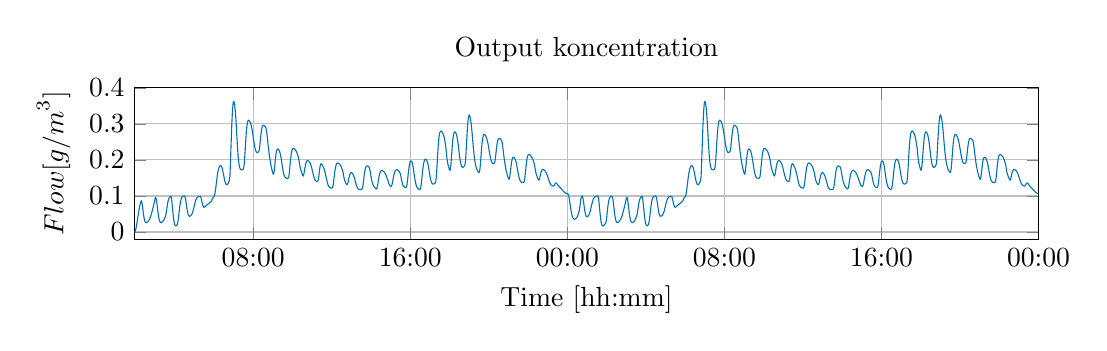
\begin{tikzpicture}

\begin{axis}[%
width=4.521in,
height=.7566in,
at={(2.6in,1.103in)},
scale only axis,
xmin=7000,
xmax=172801,
scaled x ticks = false,
xtick={1,28801,57601,86401,115201,144001,172801},
xticklabels={{00:00},{08:00},{16:00},{00:00},{08:00},{16:00},{00:00},{},{},{}},
xlabel={Time [hh:mm]},
xmajorgrids,
ymin=-0.02,
title={Output koncentration},
ymax=0.4,
ylabel={$\text{Flow [g/m}^\text{3}\text{]}$},
ymajorgrids,
axis background/.style={fill=white}
]
\addplot [color=mycolor1,solid,forget plot]
  table[row sep=crcr]{%
1	0\\
121	2.76444442474818e-109\\
241	3.26073009656065e-101\\
361	1.48722057706843e-94\\
481	9.07390854028621e-89\\
601	1.30076980586151e-83\\
701	1.08231091808059e-79\\
821	2.34738673163703e-75\\
941	1.3221333746199e-71\\
1061	3.20198537091244e-68\\
1181	5.82305692307098e-65\\
1281	2.4454529018171e-62\\
1401	2.56257479015984e-59\\
1521	1.86758071874072e-56\\
1641	9.43803249298235e-54\\
1761	3.39269645825311e-51\\
1861	3.59818145508685e-49\\
1981	7.43145424886407e-47\\
2101	1.16307577120233e-44\\
2221	1.36721652521903e-42\\
2341	1.68660368903054e-40\\
2441	2.35170957410801e-38\\
2561	1.30216127876707e-35\\
2681	5.85644996006396e-33\\
2801	2.24306122131333e-30\\
2921	7.60106686999932e-28\\
3021	9.43709554482937e-26\\
3141	5.90013951008352e-24\\
3261	1.46846532824227e-22\\
3381	2.2857813314748e-21\\
3501	1.97863169905587e-20\\
3601	7.73043630786215e-20\\
3721	2.56726045688387e-19\\
3841	6.26014920021868e-19\\
3961	1.31614841955074e-18\\
4081	2.72131669579753e-18\\
4201	6.30987738515826e-18\\
4301	1.51616521416971e-17\\
4421	5.60851788410215e-17\\
4541	2.6339333933766e-16\\
4661	1.44015306390873e-15\\
4781	8.3680115338951e-15\\
4881	3.58922621658711e-14\\
5001	1.95645240511166e-13\\
5121	9.94480128372167e-13\\
5241	4.70720404733287e-12\\
5361	2.09076018752307e-11\\
5461	7.41644489455555e-11\\
5581	7.24214793184579e-10\\
5701	3.19707992924011e-08\\
5821	5.70608545570831e-07\\
5941	1.80415957151033e-06\\
6041	3.81554329006679e-06\\
6161	8.96025772167814e-06\\
6281	2.05370658114337e-05\\
6401	4.18604942471306e-05\\
6521	7.2710127704623e-05\\
6621	0.000104304049087269\\
6741	0.000148111320476602\\
6861	0.000200586684032383\\
6981	0.000293352401992236\\
7101	0.000803797805528758\\
7201	0.00373316427553855\\
7321	0.0112988676031603\\
7441	0.0216265958635804\\
7561	0.0335097595848744\\
7681	0.0456943510219533\\
7801	0.0571866413478213\\
7901	0.0657777879623588\\
8021	0.0746358522261538\\
8141	0.0817601962521725\\
8261	0.0863572379239651\\
8281	0.0865351944787299\\
8381	0.0826868352217583\\
8481	0.0729328729720781\\
8601	0.0581850217639591\\
8721	0.044725357603887\\
8841	0.0349653661350658\\
8961	0.0291117635460206\\
9061	0.0266879469917678\\
9181	0.0258176888199261\\
9301	0.0263465314669768\\
9421	0.0277559180191354\\
9541	0.0297924228569586\\
9641	0.0319095831763245\\
9761	0.0350096550170574\\
9881	0.0388979610481673\\
10001	0.0437850540515898\\
10121	0.0497235509226516\\
10221	0.0553393938893703\\
10341	0.0625459979732243\\
10461	0.0698120774104384\\
10581	0.0767734203868196\\
10701	0.0856814291484519\\
10801	0.0926672708924115\\
10921	0.0958384827779321\\
11041	0.0900904191980293\\
11161	0.0769023939612189\\
11281	0.0611460041273074\\
11401	0.0469646731364804\\
11501	0.0380020148584435\\
11621	0.0309441692446212\\
11741	0.0273062648604276\\
11861	0.0261019009205255\\
11881	0.0260683183108994\\
11981	0.0264142750430167\\
12081	0.0274151105189277\\
12201	0.0292408712994812\\
12321	0.0316333360010084\\
12441	0.0346201085339089\\
12561	0.0383691355726851\\
12661	0.0422572667088365\\
12781	0.0482707642453505\\
12901	0.0586878405116733\\
13021	0.0720749340657065\\
13141	0.0827154885680492\\
13241	0.0890266252514835\\
13361	0.0939938169869922\\
13481	0.0968879064001237\\
13601	0.0984353528010755\\
13681	0.098813076786567\\
13721	0.0985348075014154\\
13821	0.0920427152472036\\
13941	0.075298872422749\\
14061	0.0558640981645994\\
14181	0.0387744884664413\\
14301	0.0267587617468617\\
14401	0.0208505283618553\\
14521	0.0176859050948064\\
14601	0.0171756347194794\\
14641	0.0172450864809872\\
14761	0.0184330083529576\\
14881	0.021446006624673\\
15001	0.0296915590538805\\
15101	0.0411250864689163\\
15221	0.0570253559853099\\
15341	0.0720784400230032\\
15461	0.0838664180283296\\
15581	0.0916844984904187\\
15681	0.0955974324496832\\
15801	0.0981331548392821\\
15921	0.0992804902052318\\
16041	0.0997381701301001\\
16121	0.0998281957990698\\
16161	0.0997895878738131\\
16261	0.0987248170524495\\
16381	0.0922400150811175\\
16501	0.0807971195713268\\
16621	0.0676300350816622\\
16741	0.0563839869388142\\
16841	0.0498732752106481\\
16961	0.0454520402678986\\
17081	0.043803653695271\\
17121	0.0436862670521838\\
17201	0.0439124307957137\\
17321	0.0451172938670885\\
17421	0.0467706947342416\\
17541	0.0496130963654136\\
17661	0.0537529616926854\\
17781	0.0595329505449419\\
17901	0.0667566967582858\\
18001	0.0732942416336339\\
18121	0.0808092376522041\\
18241	0.0871209626258829\\
18361	0.0918274376970769\\
18481	0.0949946886522725\\
18601	0.096941432295222\\
18701	0.0979007717822553\\
18821	0.0985342103493651\\
18941	0.0988213011868767\\
19021	0.0988838206502504\\
19061	0.0988634962711278\\
19181	0.0973930870815826\\
19281	0.091820003039776\\
19401	0.0832884205445895\\
19521	0.0755208977191211\\
19641	0.0705093124587236\\
19761	0.0686969434456523\\
19781	0.0686581463141937\\
19861	0.069028636703792\\
19981	0.0704887651006929\\
20101	0.0722625828888848\\
20221	0.0739834574284226\\
20341	0.0755580487674279\\
20441	0.0767629098487123\\
20561	0.078119337603574\\
20681	0.0794456720437077\\
20801	0.0808419954283449\\
20921	0.0824217880713266\\
21021	0.0839297245223279\\
21141	0.0860207744781929\\
21261	0.0898616104111471\\
21381	0.094105463313591\\
21501	0.0966445624733291\\
21601	0.0981197156835501\\
21721	0.102235546964558\\
21841	0.112129540365941\\
21961	0.12605362214973\\
22081	0.141321077674951\\
22201	0.15530552000296\\
22301	0.165061165884014\\
22421	0.174179084932181\\
22541	0.180230638075287\\
22661	0.183465745680596\\
22781	0.184434296028901\\
22881	0.183739374849786\\
23001	0.181005509135909\\
23121	0.17581923070715\\
23241	0.168138344869129\\
23361	0.158781849473533\\
23461	0.150759823566521\\
23581	0.142208756037235\\
23701	0.135881187917368\\
23821	0.132230364372004\\
23941	0.131130031839158\\
24041	0.131846886458409\\
24161	0.134221342645957\\
24281	0.13782272928218\\
24401	0.142486652793004\\
24521	0.154054375188698\\
24621	0.190959276274271\\
24741	0.245205232480758\\
24861	0.295861511812221\\
24981	0.333959414916128\\
25101	0.356370928796083\\
25201	0.362400038612471\\
25221	0.362449227844972\\
25321	0.358558336352734\\
25441	0.34656215833316\\
25561	0.326286055306966\\
25681	0.297589785657611\\
25801	0.264344023267989\\
25901	0.237636310542211\\
26021	0.211249512533777\\
26141	0.192934030413059\\
26261	0.181874908234323\\
26381	0.17598251860991\\
26481	0.173569857472627\\
26601	0.172443804646804\\
26661	0.172340339924044\\
26721	0.172446936843953\\
26841	0.173122047083024\\
26961	0.174423946408175\\
27061	0.177881861677216\\
27181	0.19457685767797\\
27301	0.222179251344584\\
27421	0.252857116716482\\
27541	0.279006975955229\\
27641	0.294398262045764\\
27761	0.305257376056342\\
27881	0.309743313529039\\
27961	0.310363764805266\\
28001	0.310189595932031\\
28121	0.308298112651378\\
28221	0.30550560875377\\
28341	0.30077740943752\\
28461	0.294149472214426\\
28581	0.285103013157337\\
28701	0.273760271999224\\
28801	0.26325111097251\\
28921	0.250641721541545\\
29041	0.239415061043866\\
29161	0.230613195677043\\
29281	0.224655350174716\\
29401	0.221401036313713\\
29501	0.220402566991141\\
29541	0.220352308570717\\
29621	0.220722928794362\\
29741	0.222164715112768\\
29861	0.224910230644686\\
29981	0.237004287914564\\
30081	0.25197894954146\\
30201	0.26947746203323\\
30321	0.283212177400575\\
30441	0.291688241189471\\
30561	0.295461523588751\\
30661	0.296144165483163\\
30781	0.295390894574562\\
30901	0.293799003293314\\
31021	0.29166144491173\\
31141	0.288114941178216\\
31241	0.28025659262562\\
31361	0.265232903817847\\
31481	0.248328749647045\\
31601	0.231881487962185\\
31721	0.217077755073808\\
31821	0.206165766758145\\
31941	0.194601332299876\\
32061	0.184483894414564\\
32181	0.175704716664847\\
32301	0.168268279604855\\
32401	0.163257741033995\\
32501	0.160533155403223\\
32521	0.160704787694308\\
32641	0.169069938537596\\
32761	0.186165535156872\\
32881	0.204707098149095\\
33001	0.218959384889719\\
33101	0.226206176709738\\
33221	0.230089532906655\\
33301	0.230574170469499\\
33341	0.230381426026662\\
33461	0.22857152104133\\
33581	0.225247979250713\\
33681	0.221158147397813\\
33801	0.213993289040051\\
33921	0.204018884006892\\
34041	0.192068348437596\\
34161	0.179843946989063\\
34261	0.170700116555285\\
34381	0.161945051628519\\
34501	0.155872957783439\\
34621	0.152133897013863\\
34741	0.150104683300799\\
34841	0.149287601280144\\
34961	0.148967437341586\\
34981	0.148963556713094\\
35081	0.149100170834221\\
35201	0.149635402067089\\
35321	0.153257198710477\\
35421	0.165240606342631\\
35541	0.184399688743802\\
35661	0.203419869189687\\
35781	0.218076972798879\\
35901	0.227016064682697\\
36001	0.23069821443112\\
36121	0.232113467287479\\
36141	0.23214226040682\\
36241	0.231728685638816\\
36361	0.230408998964677\\
36481	0.228504339055521\\
36601	0.226072298733475\\
36701	0.223524720845147\\
36821	0.219550171804097\\
36941	0.21432880171776\\
37061	0.207964365497901\\
37181	0.199938116335806\\
37281	0.18966011722188\\
37401	0.17987765400728\\
37521	0.172900466814579\\
37641	0.167146540269181\\
37761	0.161868058659228\\
37861	0.15778374822096\\
37961	0.155524599992351\\
37981	0.155722022791258\\
38101	0.161563826339077\\
38221	0.172361400511875\\
38341	0.183266025455923\\
38441	0.190210219111162\\
38561	0.195435705297605\\
38681	0.197845003232295\\
38781	0.19831702272898\\
38801	0.198287833444919\\
38921	0.197456733799869\\
39021	0.196053409276952\\
39141	0.193578211653186\\
39261	0.190061767603159\\
39381	0.185174650340202\\
39501	0.178803690219295\\
39601	0.172613496742503\\
39721	0.164761931019481\\
39841	0.157273333373539\\
39961	0.150901346639528\\
40081	0.14608399179095\\
40201	0.142896890010242\\
40301	0.141349413330753\\
40421	0.140545815515901\\
40481	0.140476830392724\\
40541	0.140581677343265\\
40661	0.141357193242881\\
40781	0.14829499045621\\
40881	0.16215463176129\\
41001	0.177310697625528\\
41121	0.18643618865635\\
41241	0.189352929679984\\
41261	0.189381692068831\\
41361	0.188218927961049\\
41461	0.185687662657421\\
41581	0.182131489605975\\
41701	0.17840351946569\\
41821	0.173829269058885\\
41941	0.167662560249501\\
42041	0.161269787077822\\
42161	0.152674067949021\\
42281	0.144103925471601\\
42401	0.136629195329265\\
42521	0.130878232015858\\
42621	0.127465531162475\\
42741	0.124770652300076\\
42861	0.123199225306756\\
42981	0.122368684239336\\
43101	0.122011523462945\\
43161	0.121961669276891\\
43201	0.121976114909382\\
43321	0.122657046477994\\
43441	0.129250858057506\\
43561	0.142599632895036\\
43681	0.158152267805625\\
43801	0.172038684923018\\
43901	0.180673107591385\\
44021	0.187247540583869\\
44141	0.190429779191366\\
44261	0.191362910256903\\
44281	0.19137338978929\\
44381	0.191000071862703\\
44481	0.190096520450621\\
44601	0.18850243241025\\
44721	0.186399706585078\\
44841	0.183665747644786\\
44961	0.180030708272319\\
45061	0.176147443129934\\
45181	0.170509595273739\\
45301	0.163671875801723\\
45421	0.152557206176753\\
45541	0.144167057173425\\
45641	0.13977353708981\\
45761	0.136000964153427\\
45881	0.13293299401527\\
45981	0.131312697952015\\
46001	0.131313884289518\\
46121	0.134553626264236\\
46221	0.14075560796039\\
46341	0.149660221944227\\
46461	0.157200937507326\\
46581	0.162037529999454\\
46701	0.164400201352814\\
46781	0.164853174913647\\
46801	0.164832944137965\\
46921	0.163632767214168\\
47041	0.161107698352983\\
47161	0.157785010982712\\
47281	0.153281217945739\\
47401	0.147262143674965\\
47501	0.141474810042095\\
47621	0.134499314805761\\
47741	0.128401024389963\\
47861	0.12373798716792\\
47981	0.120599340442698\\
48081	0.118991743735239\\
48201	0.117979589203081\\
48321	0.117658930644392\\
48341	0.11765348402296\\
48441	0.117774121913079\\
48561	0.118154729039946\\
48661	0.118612798373225\\
48781	0.119682334701675\\
48901	0.127232587120486\\
49021	0.141559719128736\\
49141	0.156819004579974\\
49241	0.167622204077935\\
49361	0.176688597899813\\
49481	0.181565089507746\\
49601	0.18337135604781\\
49661	0.183556136628811\\
49721	0.183439751592704\\
49821	0.182793720121873\\
49941	0.181489621315064\\
50061	0.179292468636039\\
50181	0.172893329321038\\
50301	0.162412387719161\\
50401	0.153420083023936\\
50521	0.143985214617625\\
50641	0.136721234384497\\
50761	0.131464654692538\\
50881	0.127676879895888\\
51001	0.124842200464449\\
51101	0.122949382333449\\
51221	0.121075702955252\\
51341	0.119702805070356\\
51381	0.11952788265263\\
51461	0.120716992363927\\
51581	0.12766532233538\\
51681	0.136583895433063\\
51801	0.148144476204113\\
51921	0.157925317147659\\
52041	0.164700558713691\\
52161	0.168620683096674\\
52261	0.170180595157329\\
52381	0.170677176967025\\
52501	0.170226748345767\\
52621	0.16915012086271\\
52741	0.167568895953961\\
52841	0.165844326380381\\
52961	0.163147803253587\\
53081	0.159590621531531\\
53201	0.155148956105837\\
53321	0.150059524207688\\
53421	0.145636829658566\\
53541	0.140525708619248\\
53661	0.135029925699036\\
53781	0.13032095290372\\
53901	0.128026993107315\\
54001	0.126986151207112\\
54081	0.126662727796166\\
54121	0.126949573163973\\
54241	0.131171911948409\\
54361	0.139597528008769\\
54481	0.149795028367627\\
54601	0.159042032643331\\
54701	0.164928062108658\\
54821	0.169635112726718\\
54941	0.172127887208575\\
55061	0.172994115278823\\
55101	0.173023610835978\\
55181	0.172790026536906\\
55281	0.172054811642347\\
55401	0.170636194296596\\
55521	0.168636785371471\\
55641	0.165873358462534\\
55761	0.161591393280517\\
55861	0.154945457589166\\
55981	0.14528255795534\\
56101	0.137117979905838\\
56221	0.131223505102841\\
56341	0.127439560179417\\
56441	0.12553152169543\\
56561	0.124267082250608\\
56681	0.123715381526299\\
56761	0.123612153463821\\
56801	0.123649345169826\\
56921	0.125574459273521\\
57021	0.134461836301597\\
57141	0.15022856108207\\
57261	0.167033622737534\\
57381	0.181065067033485\\
57501	0.190613078033584\\
57601	0.195155006318666\\
57721	0.197200255159215\\
57741	0.197240146127899\\
57841	0.196239725498673\\
57961	0.191985517397728\\
58081	0.183687324804279\\
58201	0.171913928877112\\
58301	0.160885308412012\\
58421	0.148307152524947\\
58541	0.138079892240592\\
58661	0.130732791778715\\
58781	0.125849879755743\\
58881	0.123126198303436\\
59001	0.120906232011767\\
59121	0.119428194568761\\
59241	0.118472256767598\\
59341	0.118145380870026\\
59361	0.118190074738609\\
59461	0.120267865608977\\
59581	0.129783707782681\\
59701	0.145741871360121\\
59821	0.163999528989139\\
59941	0.179887700365845\\
60041	0.189638893070811\\
60161	0.197272343169687\\
60281	0.201223853463956\\
60381	0.202082963570214\\
60401	0.202039719446735\\
60521	0.200721354271436\\
60621	0.198432226273931\\
60741	0.193851937215477\\
60861	0.186478498199085\\
60981	0.176311060647995\\
61101	0.164697848259418\\
61201	0.155360387373203\\
61321	0.145994118447559\\
61441	0.139343182325883\\
61561	0.135336720101241\\
61681	0.133436605596514\\
61781	0.133003197212716\\
61801	0.133010264827357\\
61901	0.13339847186403\\
62021	0.13443645130343\\
62141	0.135912797440694\\
62261	0.138541222366259\\
62381	0.154339722301692\\
62481	0.178836242950003\\
62601	0.211292720107396\\
62721	0.240005968844867\\
62841	0.260660206831289\\
62961	0.272912733404425\\
63061	0.277996008262035\\
63181	0.280119732071379\\
63221	0.280197237720685\\
63301	0.279703599901562\\
63421	0.277749967471372\\
63541	0.274632147679877\\
63641	0.27109531883942\\
63761	0.265318162934674\\
63881	0.257326314366701\\
64001	0.247066816102083\\
64121	0.234443590519152\\
64221	0.218358203366507\\
64341	0.201566790257848\\
64461	0.190609938195688\\
64581	0.182769586273719\\
64701	0.176424504069943\\
64801	0.172306467614986\\
64861	0.171263122893414\\
64921	0.173035427820021\\
65041	0.186946229213372\\
65161	0.210829530589508\\
65281	0.236421128156293\\
65401	0.256813380523448\\
65501	0.268125687282547\\
65621	0.275590723263818\\
65741	0.277930383980442\\
65761	0.277960631332574\\
65861	0.277024225430913\\
65981	0.273891658491943\\
66081	0.269551276036794\\
66201	0.26162495989936\\
66321	0.250129236285442\\
66441	0.235628215262029\\
66561	0.21997817113277\\
66661	0.207714470863248\\
66781	0.195514421608528\\
66901	0.186885687300478\\
67021	0.181798176490625\\
67141	0.179639001401567\\
67201	0.179408208085315\\
67241	0.179502658873\\
67361	0.180706719462022\\
67481	0.18289101841963\\
67601	0.185894393680798\\
67721	0.195558479239143\\
67821	0.219845153721307\\
67941	0.25390420941741\\
68061	0.285375304487389\\
68181	0.308644284808578\\
68301	0.321600782112079\\
68401	0.324286784963207\\
68521	0.321051545410977\\
68641	0.313292233347647\\
68761	0.300851856036316\\
68881	0.283241929380423\\
69001	0.262080430134431\\
69101	0.243960805487934\\
69221	0.224160279141284\\
69341	0.207946562439016\\
69461	0.195450672786006\\
69581	0.186020109400799\\
69681	0.179952105098963\\
69801	0.174316337912046\\
69921	0.170122782750927\\
70041	0.167128065066903\\
70161	0.165258695409898\\
70201	0.165016240546719\\
70261	0.165650846176839\\
70381	0.176100298851315\\
70501	0.197066600792576\\
70621	0.221926515317262\\
70741	0.243822359421681\\
70841	0.256981609930431\\
70961	0.26643264370025\\
71081	0.270432425495679\\
71161	0.271032034634726\\
71201	0.270905932464713\\
71321	0.269327819821758\\
71421	0.266964706643336\\
71541	0.262987805622455\\
71661	0.257472198389372\\
71781	0.249943849565598\\
71901	0.240370569177064\\
72001	0.231323293537346\\
72121	0.220195683975667\\
72241	0.209954075442248\\
72361	0.201564800924851\\
72481	0.195500092227108\\
72601	0.191751868977007\\
72701	0.190159930843298\\
72801	0.189663880093336\\
72821	0.189670361301948\\
72941	0.190275598812515\\
73061	0.191950729823269\\
73181	0.201341548106624\\
73281	0.215069675033658\\
73401	0.231867273588921\\
73521	0.245605371446192\\
73641	0.254492699442806\\
73761	0.258811156387285\\
73861	0.259912966033707\\
73881	0.259951612719252\\
73981	0.25956622786065\\
74101	0.258306417073047\\
74221	0.256520726262827\\
74341	0.253914467017446\\
74441	0.24857133767195\\
74561	0.235597103045261\\
74681	0.220400372217847\\
74801	0.205624000178742\\
74921	0.192574315612604\\
75021	0.183209304417277\\
75141	0.173551875557043\\
75261	0.165298324230937\\
75381	0.158234061060133\\
75501	0.15228306816584\\
75601	0.148274354365806\\
75701	0.146117355505312\\
75721	0.146274342203287\\
75841	0.153488780250664\\
75961	0.168252448561592\\
76081	0.184389354393368\\
76201	0.196919437534008\\
76301	0.203374606123165\\
76421	0.206934892116526\\
76501	0.207463906400045\\
76541	0.207344393272843\\
76661	0.205903924359296\\
76781	0.203163489345831\\
76881	0.199784113846969\\
77001	0.193856669951267\\
77121	0.185517384546372\\
77241	0.17537705119807\\
77361	0.164845896829854\\
77461	0.156857778302487\\
77581	0.149104488963247\\
77701	0.143650756305557\\
77821	0.14024859131808\\
77941	0.138377980396506\\
78041	0.137611406345773\\
78161	0.137293376050632\\
78181	0.137285411031243\\
78281	0.137386294090374\\
78401	0.137828365466121\\
78521	0.140812628801669\\
78621	0.151683575344046\\
78741	0.169543445677966\\
78861	0.187562689120253\\
78981	0.201670924948195\\
79101	0.210391891731191\\
79201	0.213998003464363\\
79321	0.215344765943397\\
79341	0.215362782406269\\
79441	0.214902506977894\\
79561	0.213555779153269\\
79681	0.211674038239239\\
79801	0.20933923834926\\
79901	0.206958218931337\\
80021	0.203319786575603\\
80141	0.198560272953762\\
80261	0.192700269209154\\
80381	0.185606843368724\\
80481	0.176051742042344\\
80601	0.165972530152896\\
80721	0.159122369734596\\
80841	0.153898093117738\\
80961	0.149383802872718\\
81061	0.145968209769426\\
81161	0.143838306485295\\
81181	0.143909600234445\\
81301	0.148009069393978\\
81421	0.15600855728772\\
81541	0.164051419679521\\
81641	0.168998531229004\\
81761	0.17239869969676\\
81881	0.173566613990258\\
81901	0.173601790696433\\
82001	0.173305994888905\\
82121	0.172219858820626\\
82221	0.170887229276094\\
82341	0.168813215454325\\
82461	0.16608663008967\\
82581	0.162459730462448\\
82701	0.157818683855372\\
82801	0.153322074528439\\
82921	0.147581597054398\\
83041	0.142020124013407\\
83161	0.137163455853173\\
83281	0.13333961119089\\
83401	0.130634005210768\\
83501	0.129157890792863\\
83621	0.128139328191677\\
83741	0.127723426242987\\
83801	0.127679537507414\\
83861	0.127735528145708\\
83981	0.129073920658983\\
84081	0.13228060884382\\
84201	0.13528013083949\\
84301	0.13610471471387\\
84321	0.13607596826055\\
84441	0.134779341972954\\
84561	0.132209603864909\\
84661	0.129845760219501\\
84781	0.127485728158148\\
84901	0.125634681000579\\
85021	0.123938669996316\\
85141	0.122154457359979\\
85241	0.120540554356715\\
85361	0.118462246897481\\
85481	0.116300692518993\\
85601	0.114173519195394\\
85721	0.112205682124206\\
85821	0.110757565491432\\
85941	0.109292774528014\\
86061	0.108126145352853\\
86181	0.107222956155136\\
86301	0.106530895557899\\
86401	0.10606781508754\\
86521	0.105396385542433\\
86641	0.101352444703132\\
86761	0.0915214974179343\\
86881	0.079013924901606\\
87001	0.0663954500967941\\
87101	0.0571574755590284\\
87221	0.0482270355502681\\
87341	0.0418474964728464\\
87461	0.0379312981931191\\
87581	0.0359613280772862\\
87681	0.0354084324459614\\
87701	0.0353925413533537\\
87801	0.0357072494607494\\
87921	0.0368298549836208\\
88041	0.0386844215744185\\
88161	0.0413382375103552\\
88261	0.0443089741033974\\
88381	0.0489852632642238\\
88501	0.0549408599599261\\
88621	0.0621805240913447\\
88741	0.0752630619824175\\
88841	0.0877733582843575\\
88961	0.0961973930661932\\
89081	0.0995362661481415\\
89121	0.0997104605364454\\
89201	0.0977193372512125\\
89321	0.088587691191014\\
89421	0.0776581082844324\\
89541	0.0640276298897265\\
89661	0.0531355694411123\\
89781	0.046296595532506\\
89901	0.0429876836994137\\
90001	0.0422884537028883\\
90121	0.0431251941842938\\
90241	0.0450162827679448\\
90361	0.0479212086862721\\
90481	0.0523336733945131\\
90601	0.0585590402551135\\
90701	0.0648561869341357\\
90821	0.0729241147950218\\
90941	0.0805426706333973\\
91061	0.0869236622005121\\
91181	0.091740756517892\\
91281	0.0946041755209932\\
91401	0.0969046832309118\\
91521	0.0982947902188968\\
91641	0.099087557460094\\
91761	0.099518107885319\\
91861	0.0997104855603433\\
91921	0.0997623623439941\\
91981	0.0996924774934149\\
92101	0.0958032592869401\\
92221	0.0799504720793797\\
92341	0.0600779459060714\\
92441	0.0444580723153603\\
92561	0.0300526548277492\\
92681	0.0213473195257541\\
92801	0.0174757970533029\\
92901	0.0166663661560637\\
92921	0.0166769738231671\\
93021	0.0173090120672348\\
93141	0.0189241943011555\\
93261	0.0211003789718111\\
93381	0.0237290078885917\\
93501	0.0278231141810732\\
93601	0.0383545077997871\\
93721	0.0565417565924759\\
93841	0.0726578301485952\\
93961	0.0844401753137214\\
94081	0.0918929424667913\\
94201	0.0960939580249704\\
94301	0.0979876416762785\\
94421	0.0991419521330638\\
94541	0.0995449099913866\\
94661	0.097654395688874\\
94781	0.0876884952362526\\
94881	0.0752907026877627\\
95001	0.059085914220699\\
95121	0.0450497285221234\\
95241	0.0350760579449971\\
95361	0.0291481765836666\\
95461	0.0267025625404729\\
95581	0.0258229929649201\\
95701	0.0263487165384103\\
95821	0.0277569516852642\\
95941	0.0297929825634608\\
96041	0.0319099518528783\\
96161	0.0350099005735165\\
96281	0.0388981383783582\\
96401	0.0437851900719673\\
96521	0.0497236600577751\\
96621	0.0553394869799584\\
96741	0.0625460762042433\\
96861	0.0698121434639444\\
96981	0.0767734754071093\\
97101	0.0856814678333269\\
97201	0.0926672940409395\\
97321	0.0958384937552925\\
97441	0.0900904225004552\\
97561	0.0769023947988\\
97681	0.061146004322035\\
97801	0.0469646731785606\\
97901	0.0380020148696363\\
98021	0.0309441692468055\\
98141	0.0273062648608521\\
98261	0.0261019009206145\\
98281	0.0260683183109688\\
98381	0.0264142750430377\\
98481	0.0274151105189347\\
98601	0.0292408712994832\\
98721	0.0316333360010091\\
98841	0.0346201085339091\\
98961	0.0383691355726852\\
99061	0.0422572667088366\\
99181	0.0482707642453505\\
99301	0.0586878405116733\\
99421	0.0720749340657065\\
99541	0.0827154885680492\\
99641	0.0890266252514835\\
99761	0.0939938169869922\\
99881	0.0968879064001237\\
100001	0.0984353528010755\\
100081	0.0988130767865669\\
100121	0.0985348075014154\\
100221	0.0920427152472036\\
100341	0.075298872422749\\
100461	0.0558640981645994\\
100581	0.0387744884664413\\
100701	0.0267587617468617\\
100801	0.0208505283618553\\
100921	0.0176859050948064\\
101001	0.0171756347194794\\
101041	0.0172450864809872\\
101161	0.0184330083529576\\
101281	0.021446006624673\\
101401	0.0296915590538805\\
101501	0.0411250864689163\\
101621	0.0570253559853099\\
101741	0.0720784400230032\\
101861	0.0838664180283296\\
101981	0.0916844984904187\\
102081	0.0955974324496832\\
102201	0.0981331548392821\\
102321	0.0992804902052318\\
102441	0.0997381701301001\\
102521	0.0998281957990698\\
102561	0.0997895878738131\\
102661	0.0987248170524495\\
102781	0.0922400150811175\\
102901	0.0807971195713268\\
103021	0.0676300350816622\\
103141	0.0563839869388142\\
103241	0.0498732752106481\\
103361	0.0454520402678986\\
103481	0.043803653695271\\
103521	0.0436862670521838\\
103601	0.0439124307957137\\
103721	0.0451172938670885\\
103821	0.0467706947342416\\
103941	0.0496130963654136\\
104061	0.0537529616926854\\
104181	0.0595329505449419\\
104301	0.0667566967582858\\
104401	0.0732942416336339\\
104521	0.0808092376522041\\
104641	0.0871209626258829\\
104761	0.0918274376970769\\
104881	0.0949946886522725\\
105001	0.096941432295222\\
105101	0.0979007717822553\\
105221	0.0985342103493651\\
105341	0.0988213011868767\\
105421	0.0988838206502504\\
105461	0.0988634962711278\\
105581	0.0973930870815826\\
105681	0.091820003039776\\
105801	0.0832884205445895\\
105921	0.0755208977191211\\
106041	0.0705093124587236\\
106161	0.0686969434456523\\
106181	0.0686581463141937\\
106261	0.069028636703792\\
106381	0.0704887651006929\\
106501	0.0722625828888848\\
106621	0.0739834574284226\\
106741	0.0755580487674279\\
106841	0.0767629098487123\\
106961	0.078119337603574\\
107081	0.0794456720437077\\
107201	0.0808419954283449\\
107321	0.0824217880713266\\
107421	0.0839297245223279\\
107541	0.0860207744781929\\
107661	0.0898616104111471\\
107781	0.094105463313591\\
107901	0.0966445624733291\\
108001	0.0981197156835501\\
108121	0.102235546964558\\
108241	0.112129540365941\\
108361	0.12605362214973\\
108481	0.141321077674951\\
108601	0.15530552000296\\
108701	0.165061165884014\\
108821	0.174179084932181\\
108941	0.180230638075287\\
109061	0.183465745680596\\
109181	0.184434296028901\\
109281	0.183739374849786\\
109401	0.181005509135909\\
109521	0.17581923070715\\
109641	0.168138344869129\\
109761	0.158781849473533\\
109861	0.150759823566521\\
109981	0.142208756037235\\
110101	0.135881187917368\\
110221	0.132230364372004\\
110341	0.131130031839158\\
110441	0.131846886458409\\
110561	0.134221342645957\\
110681	0.13782272928218\\
110801	0.142486652793004\\
110921	0.154054375188698\\
111021	0.190959276274271\\
111141	0.245205232480758\\
111261	0.295861511812221\\
111381	0.333959414916128\\
111501	0.356370928796083\\
111601	0.362400038612471\\
111621	0.362449227844972\\
111721	0.358558336352734\\
111841	0.34656215833316\\
111961	0.326286055306966\\
112081	0.297589785657611\\
112201	0.264344023267989\\
112301	0.237636310542211\\
112421	0.211249512533777\\
112541	0.192934030413059\\
112661	0.181874908234323\\
112781	0.17598251860991\\
112881	0.173569857472627\\
113001	0.172443804646804\\
113061	0.172340339924044\\
113121	0.172446936843953\\
113241	0.173122047083024\\
113361	0.174423946408175\\
113461	0.177881861677216\\
113581	0.19457685767797\\
113701	0.222179251344584\\
113821	0.252857116716482\\
113941	0.279006975955229\\
114041	0.294398262045764\\
114161	0.305257376056342\\
114281	0.309743313529039\\
114361	0.310363764805266\\
114401	0.310189595932031\\
114521	0.308298112651378\\
114621	0.30550560875377\\
114741	0.30077740943752\\
114861	0.294149472214426\\
114981	0.285103013157337\\
115101	0.273760271999224\\
115201	0.26325111097251\\
115321	0.250641721541545\\
115441	0.239415061043866\\
115561	0.230613195677043\\
115681	0.224655350174716\\
115801	0.221401036313713\\
115901	0.220402566991141\\
115941	0.220352308570717\\
116021	0.220722928794362\\
116141	0.222164715112768\\
116261	0.224910230644686\\
116381	0.237004287914564\\
116481	0.25197894954146\\
116601	0.26947746203323\\
116721	0.283212177400575\\
116841	0.291688241189471\\
116961	0.295461523588751\\
117061	0.296144165483163\\
117181	0.295390894574562\\
117301	0.293799003293314\\
117421	0.29166144491173\\
117541	0.288114941178216\\
117641	0.28025659262562\\
117761	0.265232903817847\\
117881	0.248328749647045\\
118001	0.231881487962185\\
118121	0.217077755073808\\
118221	0.206165766758145\\
118341	0.194601332299876\\
118461	0.184483894414564\\
118581	0.175704716664847\\
118701	0.168268279604855\\
118801	0.163257741033995\\
118901	0.160533155403223\\
118921	0.160704787694308\\
119041	0.169069938537596\\
119161	0.186165535156872\\
119281	0.204707098149095\\
119401	0.218959384889719\\
119501	0.226206176709738\\
119621	0.230089532906655\\
119701	0.230574170469499\\
119741	0.230381426026662\\
119861	0.22857152104133\\
119981	0.225247979250713\\
120081	0.221158147397813\\
120201	0.213993289040051\\
120321	0.204018884006892\\
120441	0.192068348437596\\
120561	0.179843946989063\\
120661	0.170700116555285\\
120781	0.161945051628519\\
120901	0.155872957783439\\
121021	0.152133897013863\\
121141	0.150104683300799\\
121241	0.149287601280144\\
121361	0.148967437341586\\
121381	0.148963556713094\\
121481	0.149100170834221\\
121601	0.149635402067089\\
121721	0.153257198710477\\
121821	0.165240606342631\\
121941	0.184399688743802\\
122061	0.203419869189687\\
122181	0.218076972798879\\
122301	0.227016064682697\\
122401	0.23069821443112\\
122521	0.232113467287479\\
122541	0.23214226040682\\
122641	0.231728685638816\\
122761	0.230408998964677\\
122881	0.228504339055521\\
123001	0.226072298733475\\
123101	0.223524720845147\\
123221	0.219550171804097\\
123341	0.21432880171776\\
123461	0.207964365497901\\
123581	0.199938116335806\\
123681	0.18966011722188\\
123801	0.17987765400728\\
123921	0.172900466814579\\
124041	0.167146540269181\\
124161	0.161868058659228\\
124261	0.15778374822096\\
124361	0.155524599992351\\
124381	0.155722022791258\\
124501	0.161563826339077\\
124621	0.172361400511875\\
124741	0.183266025455923\\
124841	0.190210219111162\\
124961	0.195435705297605\\
125081	0.197845003232295\\
125181	0.19831702272898\\
125201	0.198287833444919\\
125321	0.197456733799869\\
125421	0.196053409276952\\
125541	0.193578211653186\\
125661	0.190061767603159\\
125781	0.185174650340202\\
125901	0.178803690219295\\
126001	0.172613496742503\\
126121	0.164761931019481\\
126241	0.157273333373539\\
126361	0.150901346639528\\
126481	0.14608399179095\\
126601	0.142896890010242\\
126701	0.141349413330753\\
126821	0.140545815515901\\
126881	0.140476830392724\\
126941	0.140581677343265\\
127061	0.141357193242881\\
127181	0.14829499045621\\
127281	0.16215463176129\\
127401	0.177310697625528\\
127521	0.18643618865635\\
127641	0.189352929679984\\
127661	0.189381692068831\\
127761	0.188218927961049\\
127861	0.185687662657421\\
127981	0.182131489605975\\
128101	0.17840351946569\\
128221	0.173829269058885\\
128341	0.167662560249501\\
128441	0.161269787077822\\
128561	0.152674067949021\\
128681	0.144103925471601\\
128801	0.136629195329265\\
128921	0.130878232015858\\
129021	0.127465531162475\\
129141	0.124770652300076\\
129261	0.123199225306756\\
129381	0.122368684239336\\
129501	0.122011523462945\\
129561	0.121961669276891\\
129601	0.121976114909382\\
129721	0.122657046477994\\
129841	0.129250858057506\\
129961	0.142599632895036\\
130081	0.158152267805625\\
130201	0.172038684923018\\
130301	0.180673107591385\\
130421	0.187247540583869\\
130541	0.190429779191366\\
130661	0.191362910256903\\
130681	0.19137338978929\\
130781	0.191000071862703\\
130881	0.190096520450621\\
131001	0.18850243241025\\
131121	0.186399706585078\\
131241	0.183665747644786\\
131361	0.180030708272319\\
131461	0.176147443129934\\
131581	0.170509595273739\\
131701	0.163671875801723\\
131821	0.152557206176753\\
131941	0.144167057173425\\
132041	0.13977353708981\\
132161	0.136000964153427\\
132281	0.13293299401527\\
132381	0.131312697952015\\
132401	0.131313884289518\\
132521	0.134553626264236\\
132621	0.14075560796039\\
132741	0.149660221944227\\
132861	0.157200937507326\\
132981	0.162037529999454\\
133101	0.164400201352814\\
133181	0.164853174913647\\
133201	0.164832944137965\\
133321	0.163632767214168\\
133441	0.161107698352983\\
133561	0.157785010982712\\
133681	0.153281217945739\\
133801	0.147262143674965\\
133901	0.141474810042095\\
134021	0.134499314805761\\
134141	0.128401024389963\\
134261	0.12373798716792\\
134381	0.120599340442698\\
134481	0.118991743735239\\
134601	0.117979589203081\\
134721	0.117658930644392\\
134741	0.11765348402296\\
134841	0.117774121913079\\
134961	0.118154729039946\\
135061	0.118612798373225\\
135181	0.119682334701675\\
135301	0.127232587120486\\
135421	0.141559719128736\\
135541	0.156819004579974\\
135641	0.167622204077935\\
135761	0.176688597899813\\
135881	0.181565089507746\\
136001	0.18337135604781\\
136061	0.183556136628811\\
136121	0.183439751592704\\
136221	0.182793720121873\\
136341	0.181489621315064\\
136461	0.179292468636039\\
136581	0.172893329321038\\
136701	0.162412387719161\\
136801	0.153420083023936\\
136921	0.143985214617625\\
137041	0.136721234384497\\
137161	0.131464654692538\\
137281	0.127676879895888\\
137401	0.124842200464449\\
137501	0.122949382333449\\
137621	0.121075702955252\\
137741	0.119702805070356\\
137781	0.11952788265263\\
137861	0.120716992363927\\
137981	0.12766532233538\\
138081	0.136583895433063\\
138201	0.148144476204113\\
138321	0.157925317147659\\
138441	0.164700558713691\\
138561	0.168620683096674\\
138661	0.170180595157329\\
138781	0.170677176967025\\
138901	0.170226748345767\\
139021	0.16915012086271\\
139141	0.167568895953961\\
139241	0.165844326380381\\
139361	0.163147803253587\\
139481	0.159590621531531\\
139601	0.155148956105837\\
139721	0.150059524207688\\
139821	0.145636829658566\\
139941	0.140525708619248\\
140061	0.135029925699036\\
140181	0.13032095290372\\
140301	0.128026993107315\\
140401	0.126986151207112\\
140481	0.126662727796166\\
140521	0.126949573163973\\
140641	0.131171911948409\\
140761	0.139597528008769\\
140881	0.149795028367627\\
141001	0.159042032643331\\
141101	0.164928062108658\\
141221	0.169635112726718\\
141341	0.172127887208575\\
141461	0.172994115278823\\
141501	0.173023610835978\\
141581	0.172790026536906\\
141681	0.172054811642347\\
141801	0.170636194296596\\
141921	0.168636785371471\\
142041	0.165873358462534\\
142161	0.161591393280517\\
142261	0.154945457589166\\
142381	0.14528255795534\\
142501	0.137117979905838\\
142621	0.131223505102841\\
142741	0.127439560179417\\
142841	0.12553152169543\\
142961	0.124267082250608\\
143081	0.123715381526299\\
143161	0.123612153463821\\
143201	0.123649345169826\\
143321	0.125574459273521\\
143421	0.134461836301597\\
143541	0.15022856108207\\
143661	0.167033622737534\\
143781	0.181065067033485\\
143901	0.190613078033584\\
144001	0.195155006318666\\
144121	0.197200255159215\\
144141	0.197240146127899\\
144241	0.196239725498673\\
144361	0.191985517397728\\
144481	0.183687324804279\\
144601	0.171913928877112\\
144701	0.160885308412012\\
144821	0.148307152524947\\
144941	0.138079892240592\\
145061	0.130732791778715\\
145181	0.125849879755743\\
145281	0.123126198303436\\
145401	0.120906232011767\\
145521	0.119428194568761\\
145641	0.118472256767598\\
145741	0.118145380870026\\
145761	0.118190074738609\\
145861	0.120267865608977\\
145981	0.129783707782681\\
146101	0.145741871360121\\
146221	0.163999528989139\\
146341	0.179887700365845\\
146441	0.189638893070811\\
146561	0.197272343169687\\
146681	0.201223853463956\\
146781	0.202082963570214\\
146801	0.202039719446735\\
146921	0.200721354271436\\
147021	0.198432226273931\\
147141	0.193851937215477\\
147261	0.186478498199085\\
147381	0.176311060647995\\
147501	0.164697848259418\\
147601	0.155360387373203\\
147721	0.145994118447559\\
147841	0.139343182325883\\
147961	0.135336720101241\\
148081	0.133436605596514\\
148181	0.133003197212716\\
148201	0.133010264827357\\
148301	0.13339847186403\\
148421	0.13443645130343\\
148541	0.135912797440694\\
148661	0.138541222366259\\
148781	0.154339722301692\\
148881	0.178836242950003\\
149001	0.211292720107396\\
149121	0.240005968844867\\
149241	0.260660206831289\\
149361	0.272912733404425\\
149461	0.277996008262035\\
149581	0.280119732071379\\
149621	0.280197237720685\\
149701	0.279703599901562\\
149821	0.277749967471372\\
149941	0.274632147679877\\
150041	0.27109531883942\\
150161	0.265318162934674\\
150281	0.257326314366701\\
150401	0.247066816102083\\
150521	0.234443590519152\\
150621	0.218358203366507\\
150741	0.201566790257848\\
150861	0.190609938195688\\
150981	0.182769586273719\\
151101	0.176424504069943\\
151201	0.172306467614986\\
151261	0.171263122893414\\
151321	0.173035427820021\\
151441	0.186946229213372\\
151561	0.210829530589508\\
151681	0.236421128156293\\
151801	0.256813380523448\\
151901	0.268125687282547\\
152021	0.275590723263818\\
152141	0.277930383980442\\
152161	0.277960631332574\\
152261	0.277024225430913\\
152381	0.273891658491943\\
152481	0.269551276036794\\
152601	0.26162495989936\\
152721	0.250129236285442\\
152841	0.235628215262029\\
152961	0.21997817113277\\
153061	0.207714470863248\\
153181	0.195514421608528\\
153301	0.186885687300478\\
153421	0.181798176490625\\
153541	0.179639001401567\\
153601	0.179408208085315\\
153641	0.179502658873\\
153761	0.180706719462022\\
153881	0.18289101841963\\
154001	0.185894393680798\\
154121	0.195558479239143\\
154221	0.219845153721307\\
154341	0.25390420941741\\
154461	0.285375304487389\\
154581	0.308644284808578\\
154701	0.321600782112079\\
154801	0.324286784963207\\
154921	0.321051545410977\\
155041	0.313292233347647\\
155161	0.300851856036316\\
155281	0.283241929380423\\
155401	0.262080430134431\\
155501	0.243960805487934\\
155621	0.224160279141284\\
155741	0.207946562439016\\
155861	0.195450672786006\\
155981	0.186020109400799\\
156081	0.179952105098963\\
156201	0.174316337912046\\
156321	0.170122782750927\\
156441	0.167128065066903\\
156561	0.165258695409898\\
156601	0.165016240546719\\
156661	0.165650846176839\\
156781	0.176100298851315\\
156901	0.197066600792576\\
157021	0.221926515317262\\
157141	0.243822359421681\\
157241	0.256981609930431\\
157361	0.26643264370025\\
157481	0.270432425495679\\
157561	0.271032034634726\\
157601	0.270905932464713\\
157721	0.269327819821758\\
157821	0.266964706643336\\
157941	0.262987805622455\\
158061	0.257472198389372\\
158181	0.249943849565598\\
158301	0.240370569177064\\
158401	0.231323293537346\\
158521	0.220195683975667\\
158641	0.209954075442248\\
158761	0.201564800924851\\
158881	0.195500092227108\\
159001	0.191751868977007\\
159101	0.190159930843298\\
159201	0.189663880093336\\
159221	0.189670361301948\\
159341	0.190275598812515\\
159461	0.191950729823269\\
159581	0.201341548106624\\
159681	0.215069675033658\\
159801	0.231867273588921\\
159921	0.245605371446192\\
160041	0.254492699442806\\
160161	0.258811156387285\\
160261	0.259912966033707\\
160281	0.259951612719252\\
160381	0.25956622786065\\
160501	0.258306417073047\\
160621	0.256520726262827\\
160741	0.253914467017446\\
160841	0.24857133767195\\
160961	0.235597103045261\\
161081	0.220400372217847\\
161201	0.205624000178742\\
161321	0.192574315612604\\
161421	0.183209304417277\\
161541	0.173551875557043\\
161661	0.165298324230937\\
161781	0.158234061060133\\
161901	0.15228306816584\\
162001	0.148274354365806\\
162101	0.146117355505312\\
162121	0.146274342203287\\
162241	0.153488780250664\\
162361	0.168252448561592\\
162481	0.184389354393368\\
162601	0.196919437534008\\
162701	0.203374606123165\\
162821	0.206934892116526\\
162901	0.207463906400045\\
162941	0.207344393272843\\
163061	0.205903924359296\\
163181	0.203163489345831\\
163281	0.199784113846969\\
163401	0.193856669951267\\
163521	0.185517384546372\\
163641	0.17537705119807\\
163761	0.164845896829854\\
163861	0.156857778302487\\
163981	0.149104488963247\\
164101	0.143650756305557\\
164221	0.14024859131808\\
164341	0.138377980396506\\
164441	0.137611406345773\\
164561	0.137293376050632\\
164581	0.137285411031243\\
164681	0.137386294090374\\
164801	0.137828365466121\\
164921	0.140812628801669\\
165021	0.151683575344046\\
165141	0.169543445677966\\
165261	0.187562689120253\\
165381	0.201670924948195\\
165501	0.210391891731191\\
165601	0.213998003464363\\
165721	0.215344765943397\\
165741	0.215362782406269\\
165841	0.214902506977894\\
165961	0.213555779153269\\
166081	0.211674038239239\\
166201	0.20933923834926\\
166301	0.206958218931337\\
166421	0.203319786575603\\
166541	0.198560272953762\\
166661	0.192700269209154\\
166781	0.185606843368724\\
166881	0.176051742042344\\
167001	0.165972530152896\\
167121	0.159122369734596\\
167241	0.153898093117738\\
167361	0.149383802872718\\
167461	0.145968209769426\\
167561	0.143838306485295\\
167581	0.143909600234445\\
167701	0.148009069393978\\
167821	0.15600855728772\\
167941	0.164051419679521\\
168041	0.168998531229004\\
168161	0.17239869969676\\
168281	0.173566613990258\\
168301	0.173601790696433\\
168401	0.173305994888905\\
168521	0.172219858820626\\
168621	0.170887229276094\\
168741	0.168813215454325\\
168861	0.16608663008967\\
168981	0.162459730462448\\
169101	0.157818683855372\\
169201	0.153322074528439\\
169321	0.147581597054398\\
169441	0.142020124013407\\
169561	0.137163455853173\\
169681	0.13333961119089\\
169801	0.130634005210768\\
169901	0.129157890792863\\
170021	0.128139328191677\\
170141	0.127723426242987\\
170201	0.127679537507414\\
170261	0.127735528145708\\
170381	0.129073920658983\\
170481	0.13228060884382\\
170601	0.13528013083949\\
170701	0.13610471471387\\
170721	0.13607596826055\\
170841	0.134779341972954\\
170961	0.132209603864909\\
171061	0.129845760219501\\
171181	0.127485728158148\\
171301	0.125634681000579\\
171421	0.123938669996316\\
171541	0.122154457359979\\
171641	0.120540554356715\\
171761	0.118462246897481\\
171881	0.116300692518993\\
172001	0.114173519195394\\
172121	0.112205682124206\\
172221	0.110757565491432\\
172341	0.109292774528014\\
172461	0.108126145352853\\
172581	0.107222956155136\\
172701	0.106530895557899\\
172801	0.10606781508754\\
};
\end{axis}
\end{tikzpicture}%
\caption{Simulation of COD output of the last pipe into the WWTP.}
\label{fig:simulation_output_first_concentration}
\end{figure}  

It is clear that the flow pattern is visible in the concentration output, as it can be seen the COD amount is high in the morning when people prepares for work and low during the night as people are at sleep.  

%It can be concluded that a sewer network can be designed in the simulation model, where flow profiles and concentration can be added to the different parts of the model. Furthermore, is the simulation model able to simulate a flow and a concentration. 

A final test was conducted to investigate what a tank could do to the flow if the tank was large enough to contain the wastewater coming from the city. In this test the tank before the WWTP was increase to 300 $m^3$ with a height of 5 m and a area of 60 $m^2$.

\begin{figure}[H]
\centering
% This file was created by matlab2tikz.
%
%The latest updates can be retrieved from
%  http://www.mathworks.com/matlabcentral/fileexchange/22022-matlab2tikz-matlab2tikz
%where you can also make suggestions and rate matlab2tikz.
%
\definecolor{mycolor1}{rgb}{0.00000,0.44700,0.74100}%
%
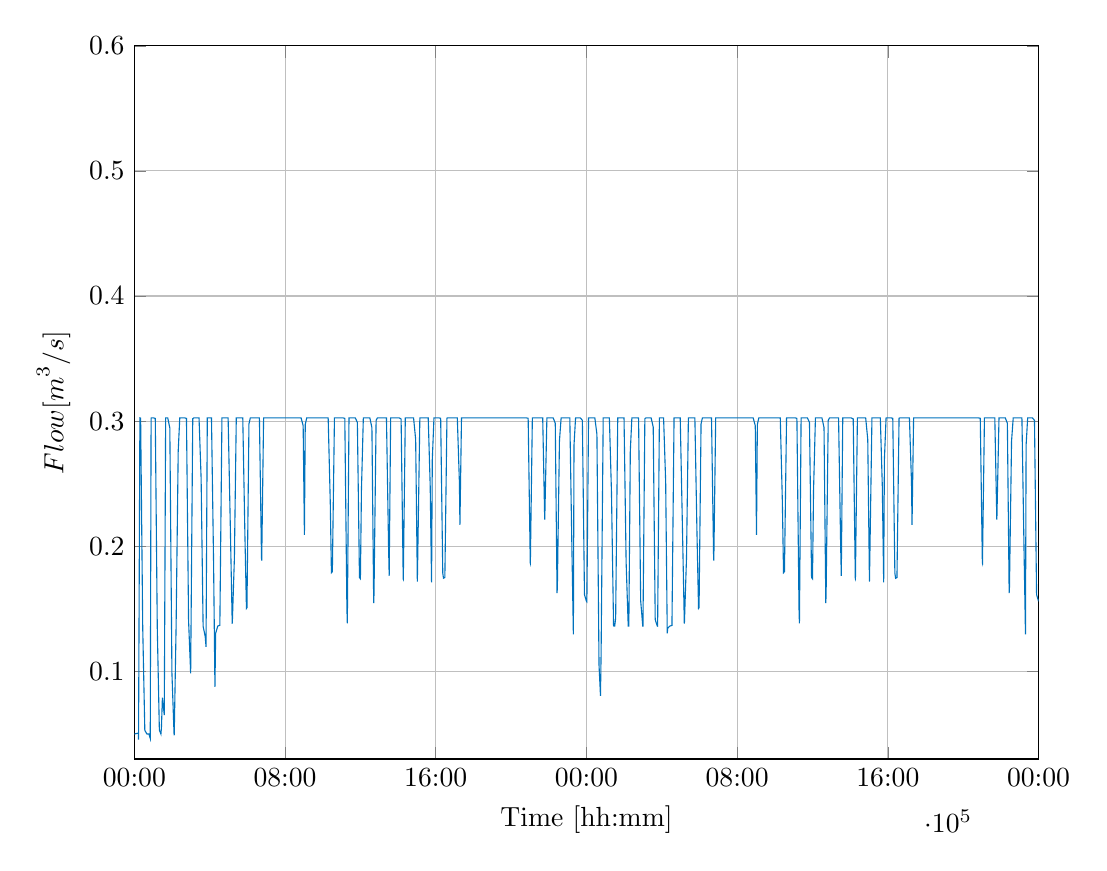
\begin{tikzpicture}

\begin{axis}[%
width=4.521in,
height=3.566in,
at={(0.758in,0.481in)},
scale only axis,
xmin=1,
xmax=172801,
xtick={1,28801,57601,86401,115201,144001,172801},
xticklabels={{00:00},{08:00},{16:00},{00:00},{08:00},{16:00},{00:00},{},{},{}},
xlabel={Time [hh:mm]},
xmajorgrids,
ymin=0.03,
ymax=0.6,
ylabel={$\text{Flow [m}^\text{3}\text{/s]}$},
ymajorgrids,
axis background/.style={fill=white}
]
\addplot [color=mycolor1,solid,forget plot]
  table[row sep=crcr]{%
1	0.0499998683647933\\
41	0.049999868172035\\
781	0.0507074272387114\\
801	0.0453941788164327\\
1061	0.302680648501631\\
1201	0.302491862717989\\
1601	0.135010674602517\\
2001	0.052887199362477\\
2401	0.0500002155001922\\
2781	0.0499999795352394\\
3041	0.0464313962055376\\
3201	0.302516352986533\\
3361	0.302680760398885\\
3601	0.302680760242387\\
4001	0.302200169403778\\
4381	0.135164719879115\\
4781	0.0530325638925076\\
5081	0.0499386124360596\\
5181	0.055586808345944\\
5361	0.0789585569468111\\
5721	0.0650508632616179\\
5981	0.302680349454319\\
6061	0.302680760387634\\
6381	0.302680760225824\\
6781	0.294520901571626\\
7181	0.0989154154146933\\
7581	0.0506834888954093\\
7621	0.0489990780965182\\
7981	0.136213836996136\\
8381	0.275956670689325\\
8681	0.302680760374472\\
8761	0.302680760242582\\
8781	0.302680760242533\\
9161	0.302680760242539\\
9561	0.302680760242384\\
9961	0.302224863193897\\
10361	0.140899783082766\\
10761	0.0983633332953129\\
11161	0.301938752023508\\
11381	0.302680760374548\\
11561	0.302680760242539\\
12081	0.302680760242539\\
12361	0.302680758907861\\
12761	0.254130778077034\\
13141	0.136059459075788\\
13541	0.127963147712897\\
13701	0.119679046615807\\
13941	0.302599210033619\\
14121	0.302680760296439\\
14341	0.302680760242539\\
14741	0.302680311240456\\
15141	0.187225056092401\\
15401	0.0875542243229154\\
15541	0.130500480790875\\
15941	0.136229862037369\\
16341	0.136809631450867\\
16741	0.302680747416122\\
16781	0.302680760373209\\
17141	0.302680760242539\\
17521	0.302680760242539\\
17921	0.302680737957046\\
18321	0.219947517927539\\
18701	0.138590577002635\\
18721	0.138604494272073\\
19121	0.190596563317006\\
19481	0.302680760292888\\
19521	0.302680760240535\\
19541	0.302680760242636\\
19921	0.302680760242539\\
20061	0.302680760242539\\
20321	0.302680760242539\\
20721	0.302680667033518\\
21121	0.210941640765384\\
21421	0.150350637668172\\
21521	0.150919846322989\\
21901	0.297770119545691\\
22161	0.302680760321777\\
22341	0.302680760242539\\
22421	0.302680760242539\\
22821	0.302680760242539\\
23001	0.302680760242539\\
23101	0.302680760242539\\
23501	0.302680760242495\\
23901	0.302537137635991\\
24301	0.190721893188483\\
24341	0.188499862099904\\
24701	0.302674453583895\\
24841	0.302680760302086\\
25101	0.302680760242539\\
25121	0.302680760242539\\
25501	0.302680760242539\\
25761	0.302680760242539\\
25901	0.302680760242539\\
25921	0.302680760242539\\
26281	0.302680760242539\\
26401	0.302680760242539\\
26681	0.302680760242539\\
26721	0.302680760242539\\
27081	0.302680760242539\\
27201	0.302680760242539\\
27481	0.302680760242539\\
27521	0.302680760242539\\
27881	0.302680760242539\\
28001	0.302680760242539\\
28281	0.302680760242539\\
28321	0.302680760242539\\
28681	0.302680760242539\\
28801	0.302680760242539\\
29081	0.302680760242539\\
29121	0.302680760242539\\
29481	0.302680760242539\\
29601	0.302680760242539\\
29881	0.302680760242539\\
29921	0.302680760242539\\
30261	0.302680760242539\\
30401	0.302680760242539\\
30661	0.302680760242539\\
30721	0.302680760242539\\
31061	0.302680760242539\\
31201	0.302680760242539\\
31461	0.302680760242539\\
31861	0.302680760226753\\
32261	0.296420028519741\\
32501	0.209173907047401\\
32661	0.297306771900499\\
32941	0.302680760303886\\
33061	0.30268076024254\\
33121	0.302680760242539\\
33461	0.302680760242539\\
33541	0.302680760242539\\
33861	0.302680760242539\\
33881	0.302680760242539\\
34261	0.302680760242539\\
34341	0.302680760242539\\
34641	0.302680760242539\\
34661	0.302680760242539\\
35041	0.302680760242539\\
35141	0.302680760242539\\
35441	0.302680760242539\\
35461	0.302680760242539\\
35841	0.302680760242539\\
35941	0.302680760242539\\
36241	0.302680760242539\\
36261	0.302680760242539\\
36641	0.302680760242539\\
37041	0.302680753339297\\
37441	0.235362546925594\\
37661	0.178862851273356\\
37841	0.179726721090916\\
38241	0.302679901182408\\
38341	0.302680760369674\\
38641	0.302680760242539\\
38681	0.302680760242539\\
39021	0.302680760242539\\
39161	0.302680760242539\\
39421	0.302680760242539\\
39821	0.302680760242383\\
40221	0.302246236787972\\
40621	0.150161908855395\\
40701	0.138355218094442\\
41021	0.302680505297797\\
41101	0.302680760397179\\
41421	0.302680760242539\\
41821	0.302680760242539\\
42221	0.302680760236874\\
42621	0.29896191150583\\
43021	0.175043157155675\\
43201	0.174045701145115\\
43401	0.245007839133707\\
43761	0.302680760291471\\
43801	0.302680760241942\\
43821	0.30268076024268\\
44201	0.302680760242539\\
44421	0.302680760242539\\
44601	0.302680760242539\\
45001	0.302680760225498\\
45401	0.294854689284065\\
45741	0.154597389404819\\
45801	0.161872632227415\\
46201	0.300594841800177\\
46461	0.302680760297433\\
46661	0.302680760242539\\
46741	0.30268076024254\\
47001	0.302680760242539\\
47121	0.302680760242539\\
47401	0.302680760242539\\
47781	0.302680760242539\\
48181	0.302679294473203\\
48581	0.200009228323768\\
48701	0.176389469603216\\
48981	0.302635857631507\\
49161	0.302680760302131\\
49441	0.30268076024254\\
49501	0.302680760242539\\
49781	0.302680760242539\\
49821	0.302680760242539\\
50181	0.302680760242539\\
50581	0.302680760241978\\
50981	0.301769350069738\\
51381	0.173914545017793\\
51401	0.173726233856688\\
51781	0.302680629822221\\
51861	0.302680760304468\\
52161	0.302680760242539\\
52201	0.302680760242539\\
52561	0.302680760242539\\
52681	0.302680760242539\\
52961	0.302680760242539\\
53361	0.302680760137084\\
53761	0.285344840884799\\
54081	0.171864139229676\\
54161	0.191627473023309\\
54561	0.302680760304719\\
54601	0.302680760241107\\
54961	0.302680760242539\\
55221	0.302680760242539\\
55361	0.302680760242539\\
55381	0.302680760242539\\
55761	0.302680760242539\\
56161	0.302680753775212\\
56541	0.248103693023625\\
56801	0.171074960948495\\
56941	0.269357952492251\\
57261	0.302680760382393\\
57361	0.302680760242545\\
57381	0.302680760242537\\
57741	0.302680760242539\\
58141	0.302680760242382\\
58541	0.302295171065643\\
58941	0.178519772866686\\
59081	0.174485379811156\\
59341	0.175023560243573\\
59741	0.302414323796332\\
59941	0.302680760295648\\
60141	0.302680760242539\\
60521	0.302680760242539\\
60921	0.302680760242539\\
61321	0.302680760242539\\
61721	0.302680757508409\\
62121	0.250916696674108\\
62221	0.217178049193355\\
62521	0.302678349363428\\
62641	0.302680760365995\\
62921	0.302680760242539\\
62941	0.302680760242539\\
63321	0.302680760242539\\
63701	0.302680760242539\\
63721	0.302680760242539\\
63861	0.302680760242539\\
64121	0.302680760242539\\
64181	0.302680760242539\\
64521	0.302680760242539\\
64661	0.302680760242539\\
64901	0.302680760242539\\
64981	0.302680760242539\\
65301	0.302680760242539\\
65321	0.302680760242539\\
65701	0.302680760242539\\
65781	0.302680760242539\\
66101	0.302680760242539\\
66121	0.302680760242539\\
66501	0.302680760242539\\
66581	0.302680760242539\\
66901	0.302680760242539\\
66921	0.302680760242539\\
67301	0.302680760242539\\
67381	0.302680760242539\\
67701	0.302680760242539\\
67721	0.302680760242539\\
68101	0.302680760242539\\
68181	0.302680760242539\\
68501	0.302680760242539\\
68521	0.302680760242539\\
68901	0.302680760242539\\
68981	0.302680760242539\\
69281	0.302680760242539\\
69301	0.302680760242539\\
69681	0.302680760242539\\
69781	0.302680760242539\\
70081	0.302680760242539\\
70101	0.302680760242539\\
70481	0.302680760242539\\
70581	0.302680760242539\\
70881	0.302680760242539\\
70901	0.302680760242539\\
71281	0.302680760242539\\
71381	0.302680760242539\\
71681	0.302680760242539\\
71701	0.302680760242539\\
72081	0.302680760242539\\
72181	0.302680760242539\\
72481	0.302680760242539\\
72501	0.302680760242539\\
72881	0.302680760242539\\
72981	0.302680760242539\\
73281	0.302680760242539\\
73301	0.302680760242539\\
73661	0.302680760242539\\
73781	0.302680760242539\\
74061	0.302680760242539\\
74101	0.302680760242539\\
74461	0.302680760242539\\
74861	0.302680760242361\\
75261	0.302311271184687\\
75661	0.18665919885132\\
75681	0.186377908093398\\
76061	0.302680540675553\\
76141	0.302680760381895\\
76461	0.302680760242539\\
76561	0.302680760242539\\
76861	0.302680760242539\\
76881	0.302680760242539\\
77261	0.302680760242539\\
77661	0.302680760242539\\
78041	0.302679346850995\\
78421	0.221375299721665\\
78441	0.222915673995048\\
78841	0.302680760370048\\
78881	0.302680760240669\\
79241	0.302680760242539\\
79341	0.302680760242539\\
79641	0.302680760242539\\
80041	0.302680760236529\\
80441	0.298307689135177\\
80781	0.162515690792454\\
80841	0.167267729521989\\
81241	0.28422427348192\\
81561	0.302680760284575\\
81641	0.302680760242527\\
81661	0.30268076024254\\
82041	0.302680760242539\\
82421	0.302680760242539\\
82841	0.302680760242539\\
83221	0.302680350128537\\
83621	0.198122368841399\\
83901	0.129520173009044\\
84021	0.280726131825289\\
84321	0.302680760283294\\
84421	0.302680760242541\\
84501	0.302680760242539\\
84961	0.302680760242539\\
85221	0.302680760240646\\
85621	0.300661703676257\\
86021	0.161380700503718\\
86401	0.155964429214595\\
86481	0.155582157734116\\
86801	0.30264576683554\\
86961	0.302680760323372\\
87201	0.302680760242539\\
87221	0.302680760242539\\
87601	0.302680760242539\\
88001	0.302680760196296\\
88401	0.289554341303737\\
88801	0.105352012864476\\
89081	0.0805055894204873\\
89201	0.114306544292461\\
89601	0.302680564793237\\
89681	0.302680760369047\\
90101	0.302680760242539\\
90301	0.302680760242539\\
90401	0.302680760242539\\
90781	0.302680757285747\\
91181	0.243263335017434\\
91581	0.136340341814795\\
91801	0.136217239567303\\
91981	0.142512616322006\\
92381	0.302680760374472\\
92421	0.302680760241047\\
92781	0.302680760242539\\
93181	0.302680760242539\\
93581	0.302679090957024\\
93981	0.187376244627345\\
94381	0.136220528223306\\
94501	0.136217239567303\\
94781	0.275956670689325\\
95081	0.302680760374472\\
95161	0.302680760242582\\
95181	0.302680760242533\\
95561	0.302680760242539\\
95961	0.302680760242503\\
96361	0.302507962825889\\
96761	0.156582670700064\\
97161	0.136217322878085\\
97201	0.136217239567303\\
97561	0.301940416259168\\
97781	0.302680760374472\\
97961	0.302680760242539\\
98061	0.302680760242539\\
98361	0.302680760242539\\
98761	0.302680760226408\\
99161	0.295215417760891\\
99541	0.141416696559254\\
99941	0.136193758336533\\
100001	0.13614720808987\\
100341	0.302668105269287\\
100481	0.302680760332779\\
100741	0.302680760242539\\
101141	0.302680758864867\\
101541	0.251403371417926\\
101841	0.130500860209357\\
101941	0.134587291476283\\
102341	0.136229862445542\\
102741	0.136809631450867\\
103141	0.302680747416122\\
103181	0.302680760373208\\
103541	0.302680760242539\\
103921	0.302680760242539\\
104321	0.302680737957046\\
104721	0.219947517927539\\
105101	0.138590577002635\\
105121	0.138604494272073\\
105521	0.190596563317006\\
105881	0.302680760292888\\
105921	0.302680760240535\\
105941	0.302680760242636\\
106321	0.302680760242539\\
106461	0.302680760242539\\
106721	0.302680760242539\\
107121	0.302680667033518\\
107521	0.210941640765384\\
107821	0.150350637668172\\
107921	0.150919846322989\\
108301	0.297770119545691\\
108561	0.302680760321777\\
108741	0.302680760242539\\
108821	0.302680760242539\\
109221	0.302680760242539\\
109401	0.302680760242539\\
109501	0.302680760242539\\
109901	0.302680760242495\\
110301	0.302537137635991\\
110701	0.190721893188483\\
110741	0.188499862099904\\
111101	0.302674453583895\\
111241	0.302680760302086\\
111501	0.302680760242539\\
111521	0.302680760242539\\
111901	0.302680760242539\\
112161	0.302680760242539\\
112301	0.302680760242539\\
112321	0.302680760242539\\
112681	0.302680760242539\\
112801	0.302680760242539\\
113081	0.302680760242539\\
113121	0.302680760242539\\
113481	0.302680760242539\\
113601	0.302680760242539\\
113881	0.302680760242539\\
113921	0.302680760242539\\
114281	0.302680760242539\\
114401	0.302680760242539\\
114681	0.302680760242539\\
114721	0.302680760242539\\
115081	0.302680760242539\\
115201	0.302680760242539\\
115481	0.302680760242539\\
115521	0.302680760242539\\
115881	0.302680760242539\\
116001	0.302680760242539\\
116281	0.302680760242539\\
116321	0.302680760242539\\
116661	0.302680760242539\\
116801	0.302680760242539\\
117061	0.302680760242539\\
117121	0.302680760242539\\
117461	0.302680760242539\\
117601	0.302680760242539\\
117861	0.302680760242539\\
118261	0.302680760226753\\
118661	0.296420028519741\\
118901	0.209173907047401\\
119061	0.297306771900499\\
119341	0.302680760303886\\
119461	0.30268076024254\\
119521	0.302680760242539\\
119861	0.302680760242539\\
119941	0.302680760242539\\
120261	0.302680760242539\\
120281	0.302680760242539\\
120661	0.302680760242539\\
120741	0.302680760242539\\
121041	0.302680760242539\\
121061	0.302680760242539\\
121441	0.302680760242539\\
121541	0.302680760242539\\
121841	0.302680760242539\\
121861	0.302680760242539\\
122241	0.302680760242539\\
122341	0.302680760242539\\
122641	0.302680760242539\\
122661	0.302680760242539\\
123041	0.302680760242539\\
123441	0.302680753339297\\
123841	0.235362546925594\\
124061	0.178862851273356\\
124241	0.179726721090916\\
124641	0.302679901182408\\
124741	0.302680760369674\\
125041	0.302680760242539\\
125081	0.302680760242539\\
125421	0.302680760242539\\
125561	0.302680760242539\\
125821	0.302680760242539\\
126221	0.302680760242383\\
126621	0.302246236787972\\
127021	0.150161908855395\\
127101	0.138355218094442\\
127421	0.302680505297797\\
127501	0.302680760397179\\
127821	0.302680760242539\\
128221	0.302680760242539\\
128621	0.302680760236874\\
129021	0.29896191150583\\
129421	0.175043157155675\\
129601	0.174045701145115\\
129801	0.245007839133707\\
130161	0.302680760291471\\
130201	0.302680760241942\\
130221	0.30268076024268\\
130601	0.302680760242539\\
130821	0.302680760242539\\
131001	0.302680760242539\\
131401	0.302680760225498\\
131801	0.294854689284065\\
132141	0.154597389404819\\
132201	0.161872632227415\\
132601	0.300594841800177\\
132861	0.302680760297433\\
133061	0.302680760242539\\
133141	0.30268076024254\\
133401	0.302680760242539\\
133521	0.302680760242539\\
133801	0.302680760242539\\
134181	0.302680760242539\\
134581	0.302679294473203\\
134981	0.200009228323768\\
135101	0.176389469603216\\
135381	0.302635857631507\\
135561	0.302680760302131\\
135841	0.30268076024254\\
135901	0.302680760242539\\
136181	0.302680760242539\\
136221	0.302680760242539\\
136581	0.302680760242539\\
136981	0.302680760241978\\
137381	0.301769350069738\\
137781	0.173914545017793\\
137801	0.173726233856688\\
138181	0.302680629822221\\
138261	0.302680760304468\\
138561	0.302680760242539\\
138601	0.302680760242539\\
138961	0.302680760242539\\
139081	0.302680760242539\\
139361	0.302680760242539\\
139761	0.302680760137084\\
140161	0.285344840884799\\
140481	0.171864139229676\\
140561	0.191627473023309\\
140961	0.302680760304719\\
141001	0.302680760241107\\
141361	0.302680760242539\\
141621	0.302680760242539\\
141761	0.302680760242539\\
141781	0.302680760242539\\
142161	0.302680760242539\\
142561	0.302680753775212\\
142941	0.248103693023625\\
143201	0.171074960948495\\
143341	0.269357952492251\\
143661	0.302680760382393\\
143761	0.302680760242545\\
143781	0.302680760242537\\
144141	0.302680760242539\\
144541	0.302680760242382\\
144941	0.302295171065643\\
145341	0.178519772866686\\
145481	0.174485379811156\\
145741	0.175023560243573\\
146141	0.302414323796332\\
146341	0.302680760295648\\
146541	0.302680760242539\\
146921	0.302680760242539\\
147321	0.302680760242539\\
147721	0.302680760242539\\
148121	0.302680757508409\\
148521	0.250916696674108\\
148621	0.217178049193355\\
148921	0.302678349363428\\
149041	0.302680760365995\\
149321	0.302680760242539\\
149341	0.302680760242539\\
149721	0.302680760242539\\
150101	0.302680760242539\\
150121	0.302680760242539\\
150261	0.302680760242539\\
150521	0.302680760242539\\
150581	0.302680760242539\\
150921	0.302680760242539\\
151061	0.302680760242539\\
151301	0.302680760242539\\
151381	0.302680760242539\\
151701	0.302680760242539\\
151721	0.302680760242539\\
152101	0.302680760242539\\
152181	0.302680760242539\\
152501	0.302680760242539\\
152521	0.302680760242539\\
152901	0.302680760242539\\
152981	0.302680760242539\\
153301	0.302680760242539\\
153321	0.302680760242539\\
153701	0.302680760242539\\
153781	0.302680760242539\\
154101	0.302680760242539\\
154121	0.302680760242539\\
154501	0.302680760242539\\
154581	0.302680760242539\\
154901	0.302680760242539\\
154921	0.302680760242539\\
155301	0.302680760242539\\
155381	0.302680760242539\\
155681	0.302680760242539\\
155701	0.302680760242539\\
156081	0.302680760242539\\
156181	0.302680760242539\\
156481	0.302680760242539\\
156501	0.302680760242539\\
156881	0.302680760242539\\
156981	0.302680760242539\\
157281	0.302680760242539\\
157301	0.302680760242539\\
157681	0.302680760242539\\
157781	0.302680760242539\\
158081	0.302680760242539\\
158101	0.302680760242539\\
158481	0.302680760242539\\
158581	0.302680760242539\\
158881	0.302680760242539\\
158901	0.302680760242539\\
159281	0.302680760242539\\
159381	0.302680760242539\\
159681	0.302680760242539\\
159701	0.302680760242539\\
160061	0.302680760242539\\
160181	0.302680760242539\\
160461	0.302680760242539\\
160501	0.302680760242539\\
160861	0.302680760242539\\
161261	0.302680760242361\\
161661	0.302311271184687\\
162061	0.18665919885132\\
162081	0.186377908093398\\
162461	0.302680540675553\\
162541	0.302680760381895\\
162861	0.302680760242539\\
162961	0.302680760242539\\
163261	0.302680760242539\\
163281	0.302680760242539\\
163661	0.302680760242539\\
164061	0.302680760242539\\
164441	0.302679346850995\\
164821	0.221375299721665\\
164841	0.222915673995048\\
165241	0.302680760370048\\
165281	0.302680760240669\\
165641	0.302680760242539\\
165741	0.302680760242539\\
166041	0.302680760242539\\
166441	0.302680760236529\\
166841	0.298307689135177\\
167181	0.162515690792454\\
167241	0.167267729521989\\
167641	0.28422427348192\\
167961	0.302680760284575\\
168041	0.302680760242527\\
168061	0.30268076024254\\
168441	0.302680760242539\\
168821	0.302680760242539\\
169241	0.302680760242539\\
169621	0.302680350128537\\
170021	0.198122368841399\\
170301	0.129520173009044\\
170421	0.280726131825289\\
170721	0.302680760283294\\
170821	0.302680760242541\\
170901	0.302680760242539\\
171361	0.302680760242539\\
171621	0.302680760240646\\
172021	0.300661703676257\\
172421	0.161380700503718\\
172801	0.155964429214595\\
};
\end{axis}
\end{tikzpicture}%
\caption{Output of the last pipe in to the WWTP, where a tank has been placed in front to smooth the flow into WWTP.}
\label{fig:simulation_output_second}
\end{figure} 
The pump has a constant output of 0,3 $m^3/s$, however if the tank is empty it will follow the flow from the input of the tank. It can be seen by comparing figure \ref{fig:simulation_output_first} and figure \ref{fig:simulation_output_second} that the top has been reduced and thereby a less fluctuated input to the WWTP is obtained.   
			   